\documentclass[11pt,a4paper]{article}
\usepackage[margin=2.5cm]{geometry}
\usepackage{amsmath,amssymb}
\usepackage{booktabs}
\usepackage{multirow}
\usepackage{graphicx}
\usepackage[colorlinks=true,linkcolor=blue,citecolor=blue,urlcolor=blue]{hyperref}
\usepackage{xcolor}
\usepackage{tikz}
\usepackage{longtable}
\usepackage{microtype}
\Urlmuskip=0mu plus 1mu
\def\UrlBreaks{\do\/\do-\do.}
\usetikzlibrary{positioning,arrows.meta,fit,backgrounds}

\newcommand{\seff}{\ensuremath{\sigma_{\mathrm{eff}}}}
\newcommand{\wait}{\textcolor{gray}{\textit{in progress}}}
\newcommand{\todo}[1]{\textcolor{red}{[#1]}}

\title{SpaceTformer: a Spacetime Transformer for Photon Energy\\
Reconstruction in the LHCb PicoCal under Pileup}
\author{Worakan Lasudee\\
\small Google Summer of Code 2026, LHCb PicoCal project}
\date{August 2026 --- draft}

\begin{document}
\maketitle

\begin{abstract}
We study photon energy regression in the proposed LHCb Upgrade~II PicoCal
electromagnetic calorimeter on a simulated minimum-bias sample, where the
photon's median share of the energy in its own cluster is $19\%$ in the
innermost region. SpaceTformer,
a token transformer over calorimeter cells --- each token a point in detector
space and time --- with a physics-constrained readout, reaches an aggregate
relative resolution $\seff = 0.0388 \pm 0.0002$, measured fully out-of-sample
under a complete ten-fold cross-validation protocol (every event predicted by
models that never saw it), a $3.2\times$ improvement over a six-feature
gradient-boosted reference on the same sample. In a paired comparison with
the encoder as the only varied component, it outperforms re-implementations
of ParticleNet and GravNet in every measured cell at every seed, at
$1.8$--$3.6\times$ their training speed --- a margin that survives a
per-baseline hyperparameter sweep. The main contribution is a
diagnosis: the resolution ceiling was set by the input window, not the
model. A seed-centred $9{\times}9$ window already holds $99.8\%$ of the
photon, so the width was not buying shower coverage: it was buying
robustness to a window centre that pileup displaces by three cells, and
above that, cells that sample the pileup field rather than the photon. The starting window held under half of the innermost region's cluster
energy, and fixing the window's size and centring cut the worst
region--energy bin by $53\%$ ($0.165 \to 0.078$), while ten encoder
families, four gate-supervision protocols, five timing constructions, a
capacity sweep and a recipe sweep all measured null against the same bins.
Two mechanisms move the number at the per-cent level: an auxiliary head
that regresses the photon's position alongside the energy, and a learned
two-stage window built on it --- a first pass points at the photon (median
error $0.16$ cells), the window is re-cut around it, a second pass
measures. On the development protocol the two-stage ensemble reads
$0.0378$ against $0.0388$, better in every one of $400$ paired resamples;
under cross-validation the same construction does not reproduce that gain,
while the auxiliary head is worth about $1\%$ under both protocols. We
report both measurements. A directly measured
data-scaling curve, $\seff \propto N^{-0.18}$ over four within-protocol
subsample points, predicts that tripling the simulated sample would bring
the aggregate to $\approx 0.033$, leaving training data as the only open
lever. The tripled-sample value is an extrapolation beyond the measured
range and is labelled as such.
\end{abstract}

\section{Introduction}

The PicoCal is the proposed electromagnetic calorimeter for LHCb
Upgrade~II~\cite{lhcbftdr}, designed to operate at instantaneous luminosities
where each photon cluster is contaminated by energy from tens of simultaneous
proton--proton interactions
\todo{state the simulated $\nu$ / luminosity --- ask the collaboration}. In
the sample used here the photon's median share of the energy inside its own
cluster is $58\%$ over all regions but only $19\%$ at 15\,mm and $32\%$ at
30\,mm: the contamination is concentrated in the small-cell inner regions. Reconstructing the photon energy then stops being a calibration
problem and becomes a separation problem. Figure~\ref{fig:pvp} makes the
statement literal: on a paired sample in which the photon's own deposit is
known cell by cell, two thirds of the energy inside the window belongs to
other interactions, and it is spread over the same cells as the photon
rather than sitting beside them.

\begin{figure}[t]
\centering
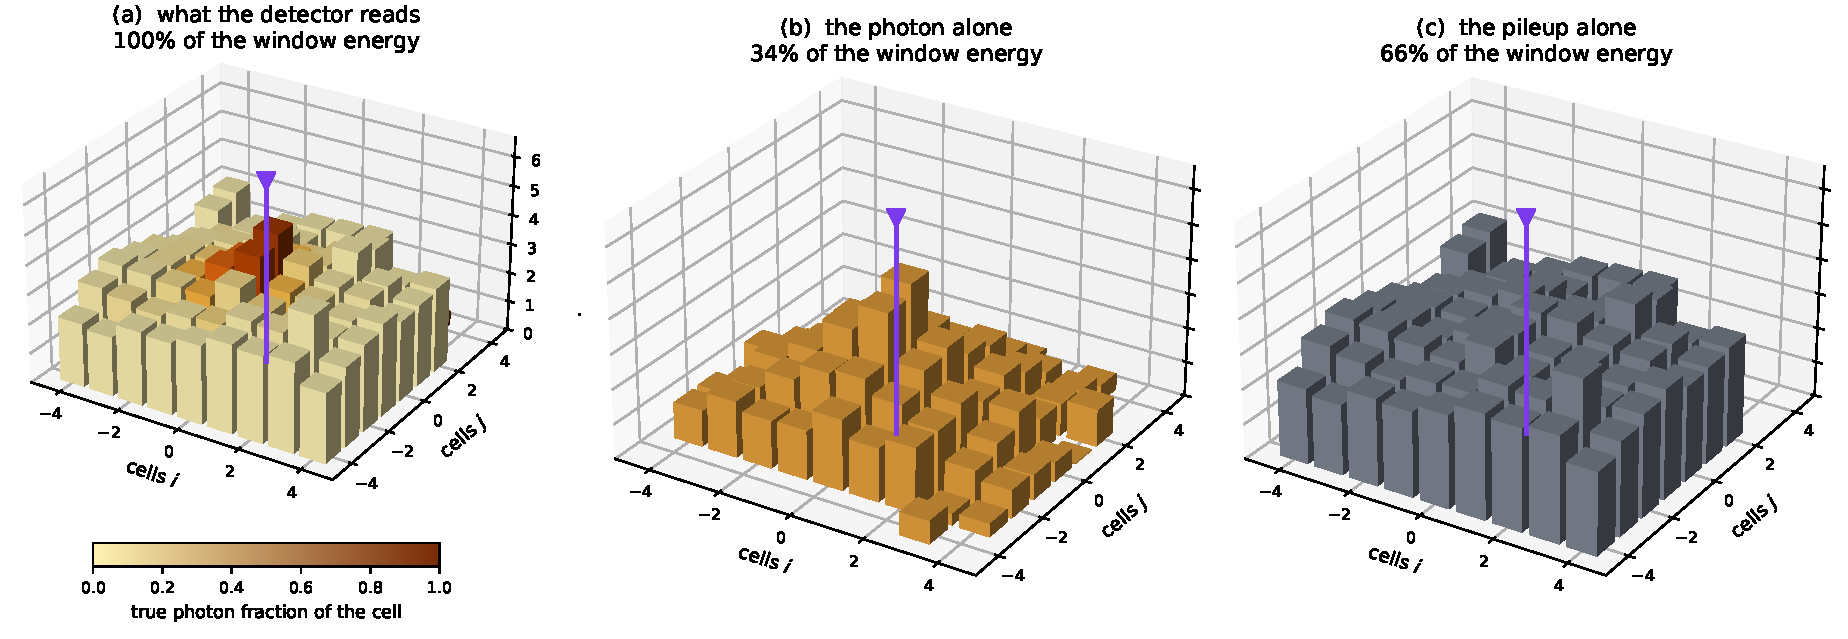
\includegraphics[width=\textwidth]{figs/photon_vs_pileup_3d.pdf}
\caption{The separation problem, on one cluster of a paired sample where
the photon's contribution to every cell is known
($15$\,mm region, $E_\gamma = 48$\,GeV). (a)~What the detector reads: bar
height is the cell energy on a logarithmic scale, colour is the fraction of
that cell which belongs to the photon. (b)~The photon's contribution alone
and (c)~the pileup contribution alone, on the same scale. The photon
supplies a third of the window energy and shares its cells with the
pileup; no cut on position or on energy separates them, which is why the
readout of Section~\ref{sec:methods} weights cells rather than selecting
them. The arrow marks the true photon entry point.}
\label{fig:pvp}
\end{figure}

Machine-learned regression is the natural tool, and the field has produced a
family of increasingly sophisticated architectures for calorimeter and jet
tasks --- graph networks such as ParticleNet~\cite{particlenet} and
GravNet~\cite{gravnet}, attention models~\cite{part}, and hybrids. Papers in
this family usually compare against numbers published on other datasets,
which makes it hard to know how much of a reported gain comes from the
architecture and how much from everything around it. We instead fix one
training protocol --- loss, splits, seeds, readout, calibration --- and vary
exactly one component at a time, treating every proposed improvement as a
hypothesis to be measured. One hundred and thirty-four distinct configurations were measured this way,
each with a saved per-event prediction set and cross-validated arms counted once (the complete scored ledger is versioned with
the code).

The thesis this discipline produced can be stated in one sentence: \emph{on
pileup-dominated PicoCal data, the resolution ceiling was set by the input
window, not the model --- widening it until it tolerated the centring error,
and then improving the centre, cut the worst bin by $53\%$, while every
architectural alternative measured null or, in the one case that attacked
the window itself, did not reproduce across protocols
(Section~\ref{sec:pointing}), leaving training-set size as the dominant
open lever.} The paper presents
the primary result and its uncertainty protocol
(Section~\ref{sec:primary}), the diagnosis with its mechanism measurements
(Sections~\ref{sec:gain}--\ref{sec:anatomy}), a quantitative account of what
now limits the measurement (Section~\ref{sec:ceiling}), the controlled architecture
campaign (Section~\ref{sec:encoders}), the record of measured negative
results (Sections~\ref{sec:gate}--\ref{sec:closed}), deployment cost
(Section~\ref{sec:cost}), and the scaling case (Section~\ref{sec:scaling}).

\section{Related work}
\label{sec:related}

\paragraph{Graph networks for irregular detectors.}
Point-cloud learning entered vision through PointNet~\cite{pointnet} and
EdgeConv~\cite{dgcnn}, and particle physics through
ParticleNet~\cite{particlenet} (EdgeConv over dynamically recomputed
$k$-nearest-neighbour graphs) and GravNet~\cite{gravnet} (aggregation
weighted by distance in a learned latent space, designed for calorimeters);
the same lineage now powers full particle-flow reconstruction
(MLPF~\cite{mlpf}) and symmetry-equivariant taggers
(LorentzNet~\cite{lorentznet}). ParticleNet and GravNet, the two most
often recommended for our task, are re-implemented and measured here under
a paired protocol (Section~\ref{sec:encoders}). We read the outcome not as
a criticism of the architectures but as evidence that at $O(10^2)$ tokens
with severe per-cell noise, local graph connectivity provides no advantage over full
attention.

\paragraph{Attention in particle physics.}
The transformer~\cite{vaswani} entered jet physics through the Particle
Transformer~\cite{part}, whose pairwise physics-motivated attention bias is
the direct ancestor of one of our losing arms.
TimeSformer~\cite{timesformer} showed that factorising attention along the
time axis is effective for video; our time-sliced attention arm transplants that idea
using per-cell time as the axis, and it loses --- video frames are dense and
redundant along time, calorimeter timestamps are one noisy scalar per token.
Patch-hierarchical attention for jets~\cite{patchjets} cuts attention cost
by grouping tokens into patches --- there consecutive chunks of a
particle list ordered by $p_\mathrm{T}$ by default, explicitly not spatial
regions. We
transplanted the cost argument to a geometry where the hierarchy can be
spatial: individual cells in the core, coarse ring summaries outside. It is
the one transplanted idea that survives measurement.
ClusTEX~\cite{clustex} separates global from local detector coordinates; the
same separation measured here is neutral.

\paragraph{Set, flow, and mixing methods.}
Deep Sets~\cite{deepsets} pool per-particle embeddings additively; Energy
Flow Networks~\cite{efn} restrict that pooling to an energy-weighted sum
over angular directions, which is what makes them infrared- and
collinear-safe --- the unrestricted Deep Sets form is not. Our EFN arm
confirms that a linear pooling of this kind is too weak when the task is
subtractive --- separating overlapping
energy fields rather than summarising one. MLP-Mixer-style token
mixing~\cite{mixer} replaces attention with a learned but
input-independent MLP across tokens; a masked Mixer arm measured here loses heavily
(Section~\ref{sec:encoders}) --- under pileup the informative cells move
event by event, which content-based attention tracks and a fixed mixing pattern
weights cannot.

\paragraph{Linear attention and state-space models.}
The Mamba lineage~\cite{mamba} offers linear-complexity sequence mixing whose
advantage is most pronounced at long sequence length (its published
comparisons run to thousands of tokens and beyond). Our events carry 81--289 tokens, where full attention
is exact and inexpensive, so we deprioritised the family without measurement and
say so explicitly.

\paragraph{Self-supervised vision backbones.}
We assessed DINOv3-style pretraining~\cite{dinov3} on cell images and
declined to run it: the pretraining distribution shares no statistics with
sparse calorimeter depositions, and our labelled sample ($7\times10^4$
events) is far below the regime where frozen-backbone transfer beats direct
training.

\paragraph{Boosted trees and calorimetry under pileup.}
Gradient-boosted decision trees~\cite{xgboost,lightgbm} remain the standard
fast baseline --- ATLAS calibrates electron and photon energies with
tree-based regression~\cite{atlascalib} --- and ours is specified in
Section~\ref{sec:data}. Learned pileup mitigation began with
PUMML~\cite{pumml} and attention-based variants~\cite{abcnet}; learned
graph-based architectures have been explored for calorimeter energy
regression in the CMS context --- dynamic graph reduction~\cite{drn} and
deep-learning clustering studies in the ECAL~\cite{cmsecaldl}.
Those works subtract pileup or regress energy; ours does both in one model
and reports where the ceiling comes from. The design of the CMS HGCAL~\cite{hgcal,hgcaltiming} rests on the same
premise as our per-bin pattern: fine transverse granularity and per-cell
timing were chosen so that overlapping showers can be separated under HL-LHC
pileup~\cite{hgcaltiming}, which is where our own improvements concentrate. The quantile (pinball) loss goes back to~\cite{koenker} and was carried
into neural networks by the statistics and forecasting
literature~\cite{white92,qrnn}; the
exponential moving average of weights used here follows the mean-teacher
form~\cite{meanteacher}, of which the equal-weight iterate averaging
of~\cite{polyak} is the classical ancestor; deep ensembles
to~\cite{deepens}.

\section{Dataset and task}
\label{sec:data}

Two simulated samples are used. The \emph{minimum-bias sample} --- the
physics target and the source of every quoted number --- contains 72{,}554
photon clusters under realistic pileup, spanning the five PicoCal cell-size
regions with photon energies restricted to 1--100\,GeV. Its region
composition (from the cross-validated half: 15\,mm $\sim$12\%, 30\,mm
$\sim$19\%, 40\,mm $\sim$29\%, 60\,mm $\sim$34\%, 120\,mm $\sim$6\%) makes
the aggregate metric outer-region dominated, a fact that matters repeatedly
below. A \emph{clean sample} of pileup-free photon showers from the same
simulation enters only as a training auxiliary
(Section~\ref{sec:methods}). Each cluster provides its cells with per-cell
energy, position, and two timestamps from the front and back longitudinal
compartments --- only $\sim$$37\%$ of cells carry a usable front timestamp ---
plus cluster-level quantities from the standard reconstruction (cluster
position, summed energy, cell multiplicity).
\todo{Simulation provenance to be completed with the collaboration:
generator and simulation framework versions, pileup conditions, out-of-time
spillover, timestamp digitisation and resolution, photon selection.} The
target is the true photon energy.

\paragraph{Figure of merit.} The effective resolution \seff{} is the
half-width of the minimal interval containing $68.3\%$ of the per-event
relative residuals $(E_{\mathrm{pred}}-E_{\mathrm{true}})/E_{\mathrm{true}}$.
It is robust to tails (Figure~\ref{fig:residuals} shows why a Gaussian fit
would not represent these distributions), and it is bias-blind, which is why
we report linearity separately (Figure~\ref{fig:linearity}).

We report \seff{} in fifteen bins --- five regions $\times$ three energy
terciles, with tercile edges anchored to the starting configuration's energy
distribution per region: 46.8/73.8\,GeV (15\,mm), 31.7/57.5\,GeV (30\,mm),
19.2/34.0\,GeV (40\,mm), 12.1/21.5\,GeV (60\,mm), 9.4/16.5\,GeV (120\,mm) ---
plus the event-weighted aggregate, and continuously versus energy in
Figure~\ref{fig:resve}.

\paragraph{Evaluation protocol.} The primary protocol is ten-fold
cross-validation with a 5\% validation slice, so each model trains on
$85.5\%$ of events. All ten folds are trained: every event in the sample is
predicted exactly once, by an ensemble of five models that never saw it,
with the per-event prediction the median over members. The five members per
fold are three seeds of the main configuration plus one member with
region-restricted recentring and one trained on all cluster cells
(Section~\ref{sec:methods}). During development we used a fixed 70/15/15
split with larger seed ensembles; that protocol biases the weak bins optimistically by
roughly $0.009$ (15\,mm low-E: $0.0691$ fixed-split vs $0.0783$
cross-validated), so we do not quote fixed-split numbers as primary results and we
label the protocol wherever one appears. Against selection effects across
the $134$-configuration campaign (scored ledger versioned with the code): the
primary protocol was fixed before the final measurement, screening runs
never enter the primary claims, and the half-sample preview and its correction
($0.0379 \to 0.0388$) are reported rather than absorbed.

\paragraph{Uncertainties.} Two kinds are quoted. On ensemble numbers: a
bootstrap error over test events (400 resamples). On claims comparing
configurations: the spread of \seff{} across independently trained members,
which is the appropriate reproducibility scale --- a pooled statistical error
would assume independent test events that repeat across members. Across the
50 member--fold arms of the primary result, a single member's aggregate
\seff{} is $0.0397$ with spread $0.0010$; in the weak bins the single-member
spread is $0.0070$ (15\,mm low-E) and $0.0046$ (30\,mm low-E).

\paragraph{GBDT reference.} The external baseline is a
histogram-based gradient-boosted regressor (300 iterations) on six summary
features per cluster --- log summed window energy, front/back energy ratio,
cell multiplicity, log seed-cell energy, energy-weighted lateral width, and
region --- trained on the same events with a log-energy target, single model,
fixed split. It reaches aggregate $\seff = 0.1253$ on this sample
(per-region curves in Figure~\ref{fig:resve}); the same-protocol
transformer improves on it by $3.2\times$. It is a fast-baseline reference,
not a tuned competitor, and we label it as such. One substitution relative
to the original project plan is made explicit: the LHCb production
clustering algorithms (the Cellular Automaton and its graph-clustering
successor) run upstream of this dataset --- the clusters we receive
\emph{are} their output --- so their energy estimate enters our comparisons
as the calibrated cluster sum ($\seff = 0.184$ on this sample,
Figure~\ref{fig:throughput}) rather than as re-implementations.

\section{Methods}
\label{sec:methods}

Figure~\ref{fig:arch} shows the full SpaceTformer pipeline. Throughout, the
\emph{seed cell} is the highest-energy cell used by the standard
reconstruction to anchor a cluster, and \emph{ring} $r$ denotes the square
shell of cells at Chebyshev distance $r$ from the window centre.

\begin{figure}[t]
\centering
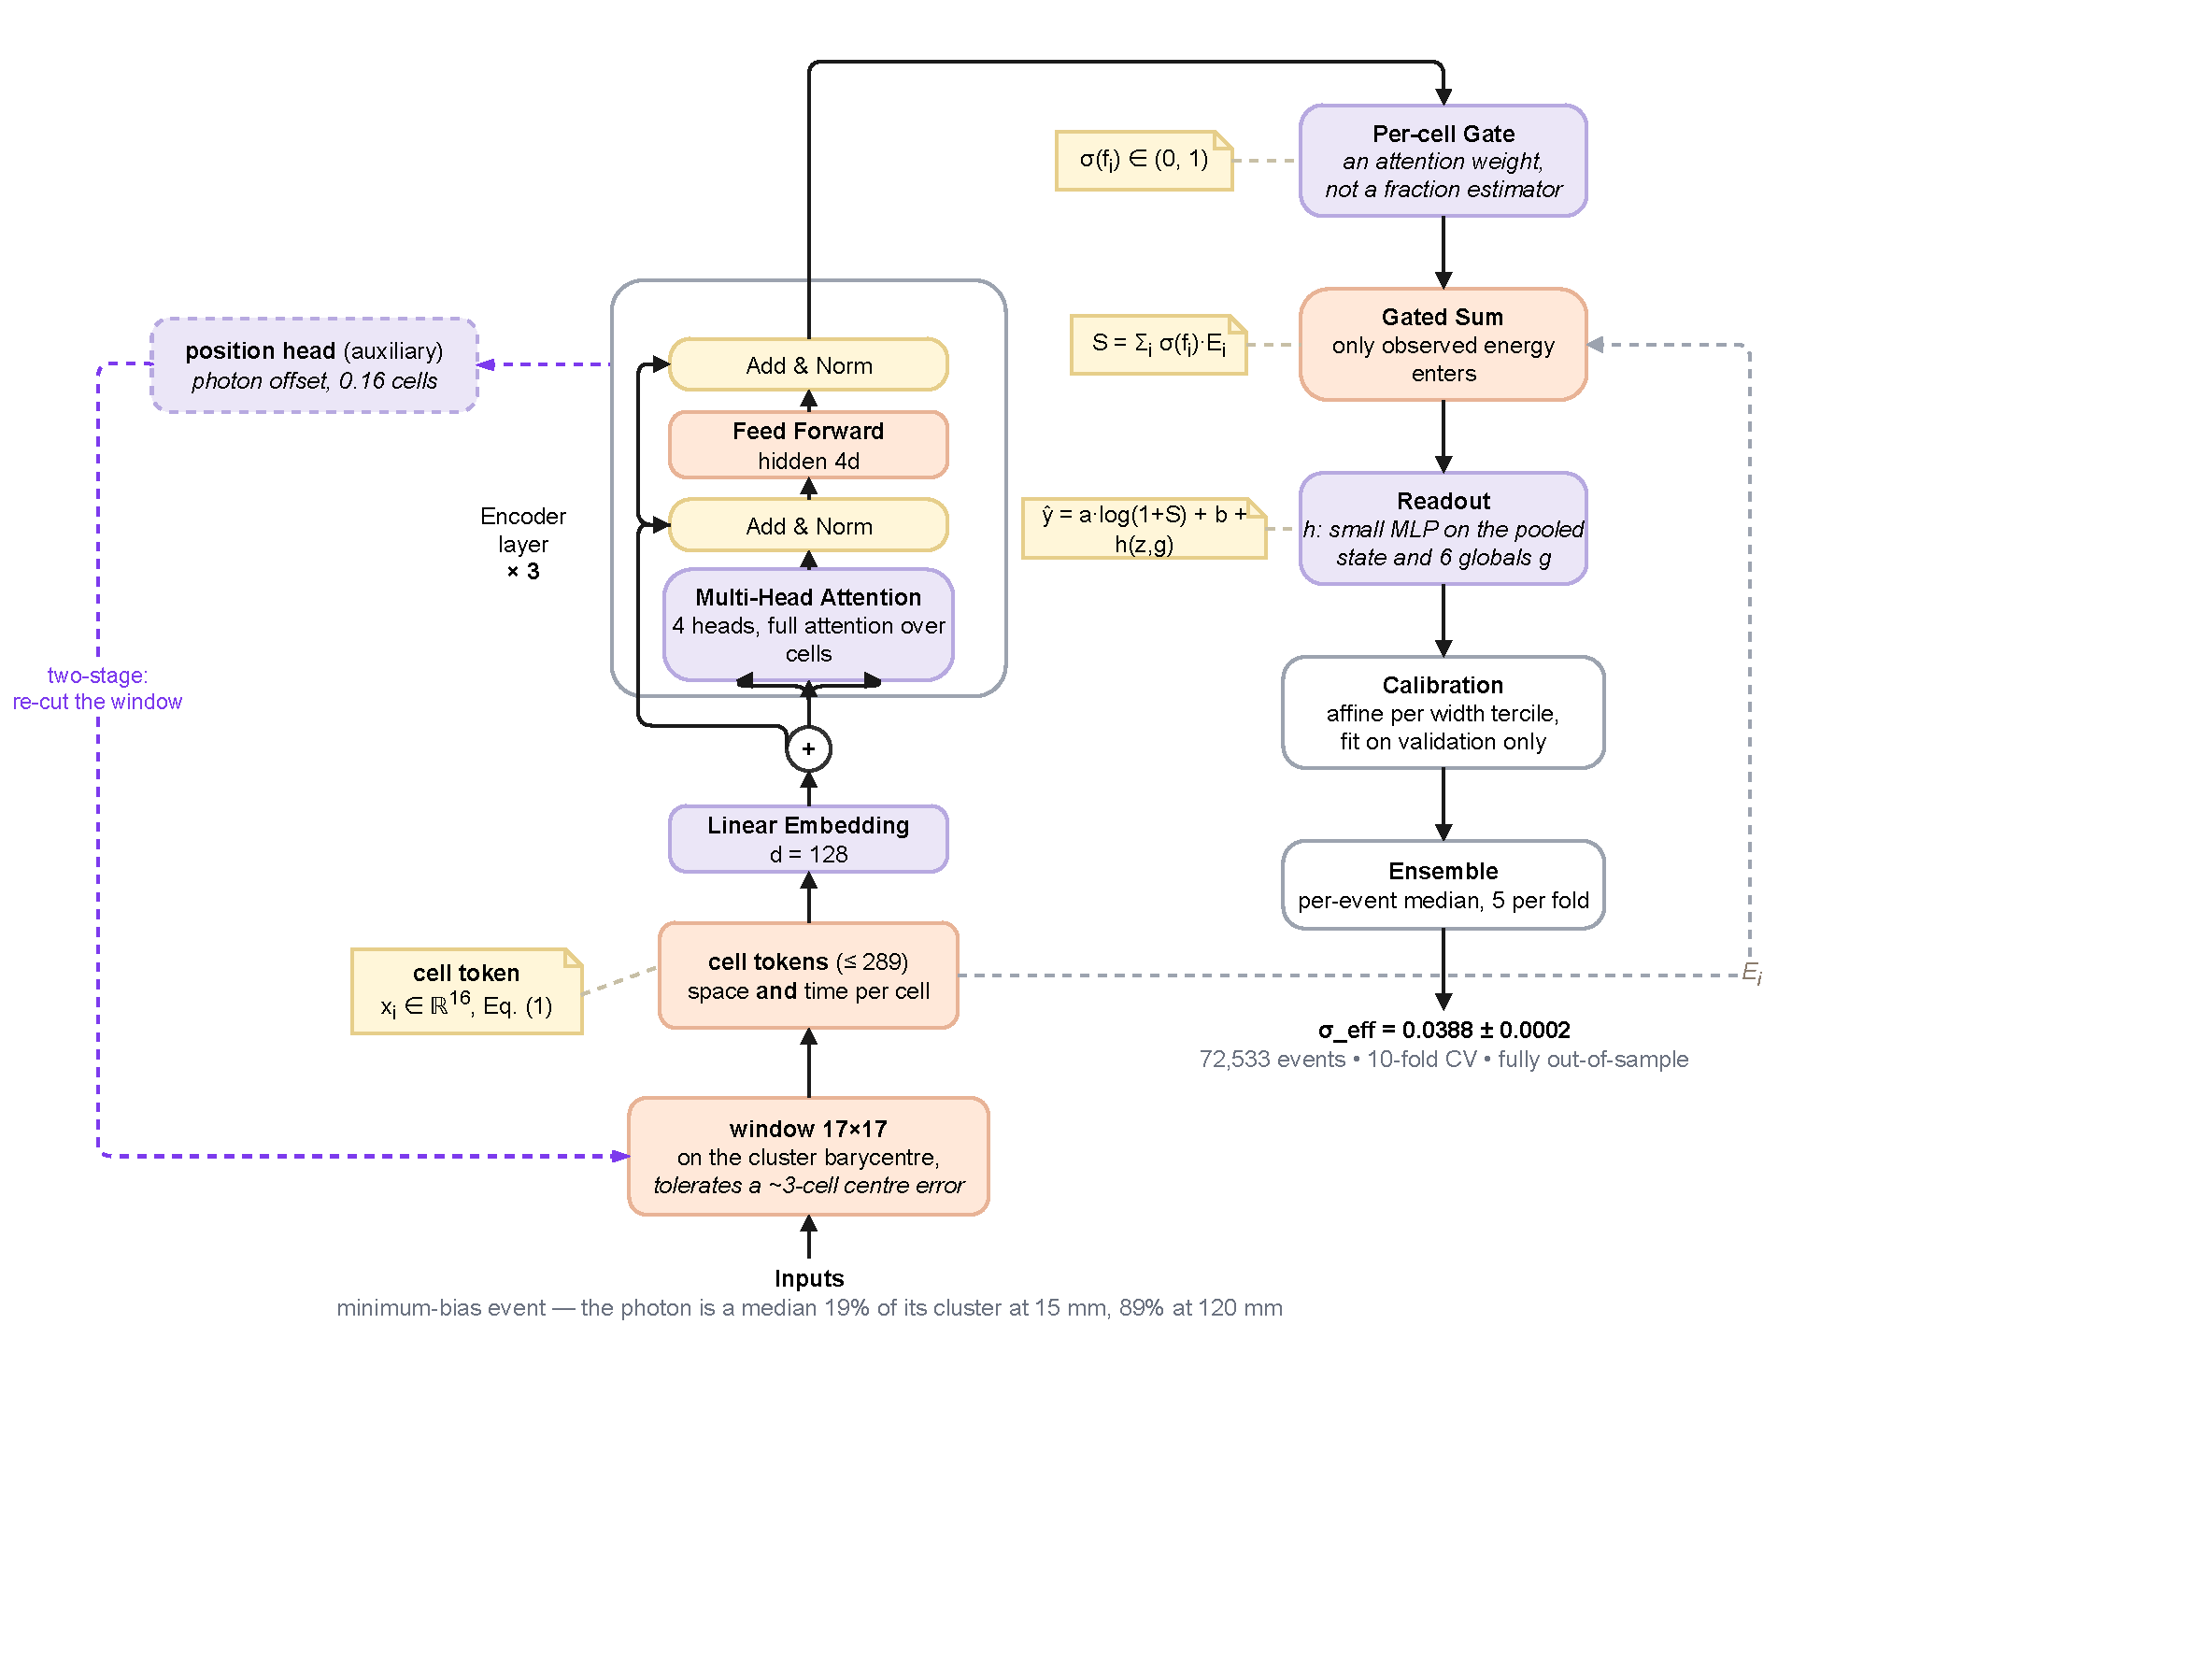
\includegraphics[width=\textwidth]{spacetformer.pdf}
\caption{The SpaceTformer pipeline. Each cell is a token in detector space
and time; the encoder is a plain transformer over cell tokens only; the
cluster-level global features $g$ enter only at the readout, which is a gated
energy sum in log space plus a small correction $h$; the loss is a three-quantile
pinball loss with EMA weights; predictions are the per-event median over
ensemble members; the inset draws $h$ itself, a one-hidden-layer network from the pooled state and the globals to the three quantiles. The decisive components are the window's size and
centring at the bottom (Section~\ref{sec:gain}). Dashed purple: the
auxiliary position head and the two-stage path that re-cuts the window
around the predicted photon position (Section~\ref{sec:pointing}).}
\label{fig:arch}
\end{figure}

\paragraph{Tokens.} Each fired calorimeter cell $i$ of the window becomes one
token of sixteen channels,
\begin{equation}
\mathbf{x}_i = \Big(
  \log(1{+}E_i),\;
  \log(1{+}E_i^{\mathrm{f}}),\;
  \log(1{+}E_i^{\mathrm{b}}),\;
  \delta_i,\; \delta_j,\; r_i,\;
  \log p,\;
  \Delta t_i^{\mathrm{f}},\; \Delta t_i^{\mathrm{b}},\;
  h_i^{\mathrm{f}},\; h_i^{\mathrm{b}},\;
  \mathbf{1}_\rho
\Big) \;\in\; \mathbb{R}^{16},
\label{eq:token}
\end{equation}
where $E_i$ is the cell energy and $E_i^{\mathrm{f}}, E_i^{\mathrm{b}}$ its
front and back longitudinal samples; $(\delta_i, \delta_j)$ is the offset from
the window centre in cells and $r_i$ its modulus; $p$ is the cell pitch;
$\Delta t_i^{\mathrm{f},\mathrm{b}} = t_i^{\mathrm{f},\mathrm{b}} -
\mathrm{med}_j\, t_j^{\mathrm{f},\mathrm{b}}$ are the two timestamps with the
window median removed and clipped to $\pm 5$\,ns;
$h_i^{\mathrm{f}}, h_i^{\mathrm{b}} \in \{0,1\}$ record whether each timestamp
exists; and $\mathbf{1}_\rho$ is a five-way one-hot of the calorimeter region.
The two time channels are arrival times, not an engineered pull: subtracting
the window median removes only the event's overall time offset. A cell with no
usable timestamp carries $h=0$ beside a zero, which after the linear embedding
is equivalent to a learnable missing-value embedding.
The whole set $\{\mathbf{x}_i\}$ is what the encoder attends over; nothing is
aggregated before it.
Cluster-level reconstruction quantities enter as global features, together
with one indicator marking events drawn from the clean auxiliary sample rather
than from minimum bias. All inputs come from the standard reconstruction or
from that sample label; none uses generator truth.
Figures~\ref{fig:input3d} and~\ref{fig:input} show the same real input from
two views: the token set as the detector produces it --- one box per fired
cell, in space, in time, and split over the two longitudinal segments ---
and the same event in projection, where the pileup blanket the model must
subtract, the sparsity of the timestamps, and the three candidate window
centres of Section~\ref{sec:gain} are read off directly.

\begin{figure}[t]
\centering
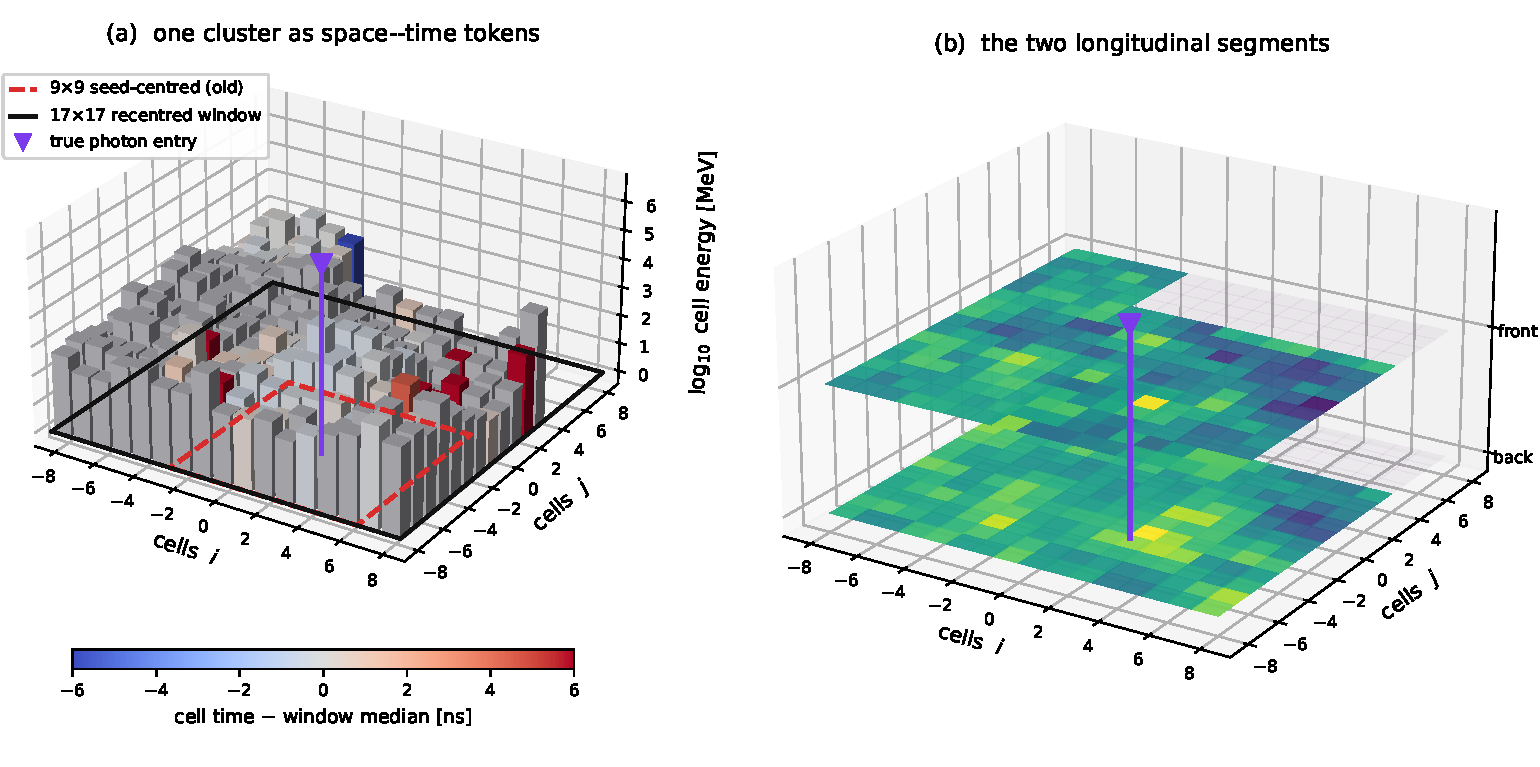
\includegraphics[width=\textwidth]{figs/event_3d.pdf}
\caption{One minimum-bias cluster as the model receives it
($15$\,mm region, $E_\gamma = 37$\,GeV, 424 fired cells). (a)~Each fired
cell is one token: its position in the $17{\times}17$ window, its energy
(bar height) and its timestamp relative to the window median (colour;
grey bars carry no timestamp). Pileup deposits fill the window at all
times, while the photon's own cells arrive together near zero. (b)~The
same cluster in its two longitudinal segments, the depth information that
separates the start of the shower from its tail.}
\label{fig:input3d}
\end{figure}

\begin{figure}[t]
\centering
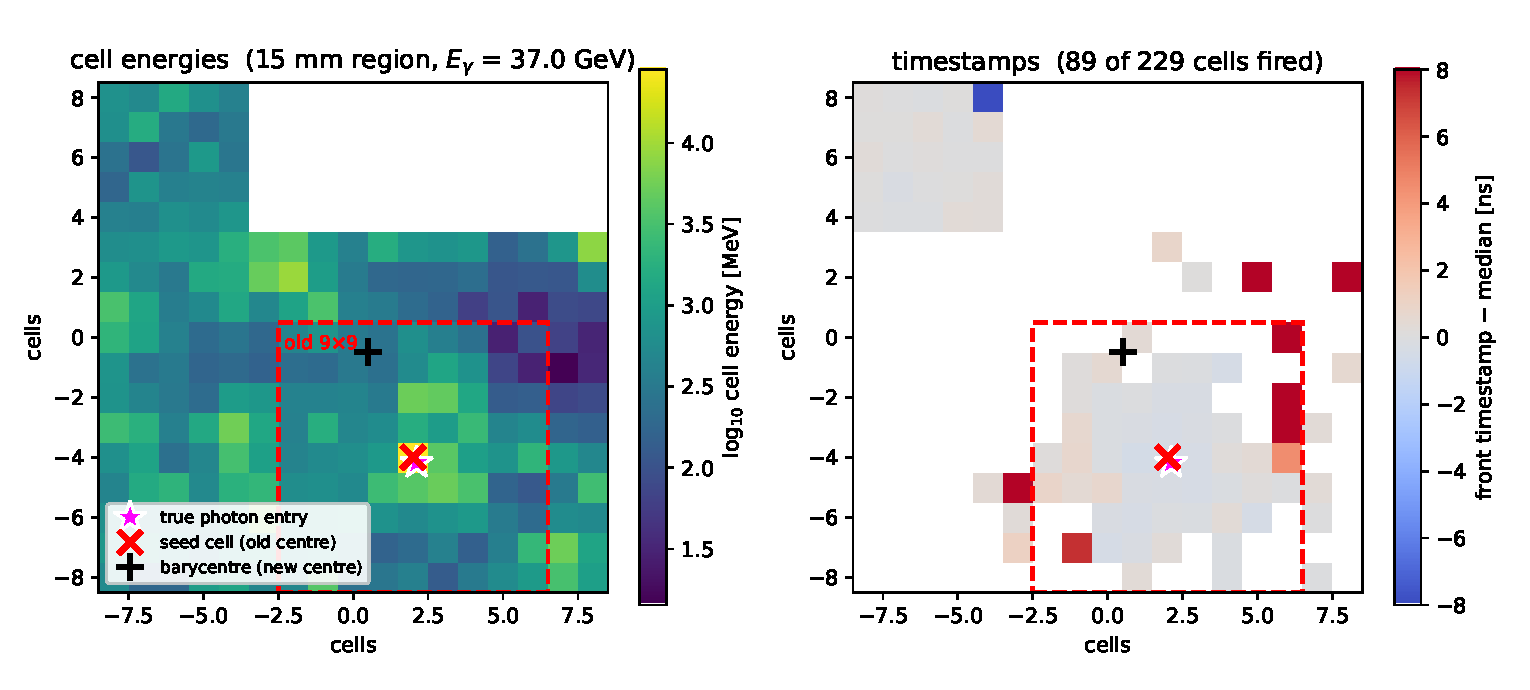
\includegraphics[width=0.96\textwidth]{figs/input_example.pdf}
\caption{One real minimum-bias input to SpaceTformer: a 15\,mm-region
cluster ($E_\gamma = 37$\,GeV, 424 cells) shown in the recentred
$17{\times}17$ window. Left: per-cell energies --- pileup deposits
everywhere, with $74\%$ of the cluster energy outside the starting
$9{\times}9$ window (red dashed). Right: front timestamps, carried by only
$39\%$ of the fired cells. Markers: true photon entry (star), seed cell
(cross, the old window centre), energy barycentre (plus, the new centre).}
\label{fig:input}
\end{figure}

\paragraph{Window.} The decisive design choices are \emph{where} the window
sits and \emph{how much} it covers, not what reads it. The main
configuration uses a $17{\times}17$ window --- half-width $w=8$ cells, so
$(2w+1)^2 = 289$ grid positions --- centred on the cluster energy
barycentre (computable from standard reconstruction quantities, hence
available online) in \emph{all} regions; one ensemble member instead
restricts the recentring to the two inner regions, where the measured
mis-seeding rate is highest and the gain concentrates.
Section~\ref{sec:gain} presents the measurements behind both choices.

\paragraph{Encoder.} SpaceTformer's encoder is a plain token
transformer~\cite{vaswani}: $d=128$, 4 heads, 3 layers, feed-forward width
$4d$, dropout 0.1, full self-attention over the cell tokens. The
six cluster-level global features do not enter the encoder; they are
concatenated to the pooled state at the readout. Attention therefore operates
on per-cell channels, with the caveat that two of them --- the cell pitch and
the region one-hot --- are constant within an event and tell the encoder which
region it is reading. The name marks what the model attends over --- each token
is a point in detector space \emph{and} time, with the timestamps worth
$20\%$ of the aggregate resolution (Section~\ref{sec:timing}) --- not a
factorised attention scheme: we measured time-factorised attention and it
loses. Ten encoder families were tried against this one
(Section~\ref{sec:encoders}); none won.

\paragraph{Physics-constrained readout.} Instead of predicting the energy
freely, the network emits a per-cell gate $\sigma(f_i)\in(0,1)$ and the
readout is
\begin{equation}
\hat{y} = a \cdot \log\!\Big(1 + \sum_i \sigma(f_i)\, E_i\Big) + b
          + h(z, g),
\label{eq:readout}
\end{equation}
a gated energy sum in log space plus a small learned correction $h$ (an MLP
on the pooled encoder state $z$ and the global features $g$). The gated sum
is the dominant pathway and anchors the prediction to observed cell
energies; the correction term is free in log space and absorbs what the sum
cannot express, so the constraint is an inductive bias, not a hard bound.
This stabilises the low-statistics bins. We stress, and measure in
Section~\ref{sec:gate}, that the learned gate is \emph{not} a per-cell
pileup-fraction estimator and forcing it to be one hurts.

\paragraph{Loss and target.} The choice was measured, not assumed
(Table~\ref{tab:loss}, all arms sharing this encoder). Predicting the energy
directly and predicting a residual on the calibrated sum are
indistinguishable and poor; the gated readout with a Huber loss halves the
error; quantile losses beat Huber. The production loss is a pinball loss at
quantiles $(0.25, 0.5, 0.75)$ --- the median is the prediction --- plus a
width-regularisation term that penalises wide inter-quantile intervals while
softly enforcing their coverage. One arm deserves its warning label:
\emph{trimmed risk} --- dropping the worst $10\%$ or $20\%$ of events from
the loss, a textbook move for a robust target metric --- is catastrophic
($0.0513$ and $0.0565$) and unstable across seeds ($\pm 0.05$ at 15\,mm
low-E). The events it drops are precisely the pileup-heavy population of
Section~\ref{sec:anatomy}; refusing to train on them removes the hard half
of the physics.

\begin{table}[h]
\centering
\caption{Loss and target study, identical encoder, fixed-split protocol,
aggregate \seff{} (five seeds unless noted).}
\label{tab:loss}
\small
\begin{tabular}{llc}
\toprule
target / loss & note & aggregate\\
\midrule
direct energy, L2 & & 0.0650\\
residual on calibrated sum, L2 & & 0.0675\\
gated readout, Huber & first structural gain & 0.0462\\
gated readout, 3-quantile & & 0.0427\\
+ EMA + clean-sample auxiliary & frozen recipe & \textbf{0.0390}\\
\midrule
trimmed risk, drop worst 10\% & 2 seeds & 0.0513\\
trimmed risk, drop worst 20\% & 2 seeds & 0.0565\\
\bottomrule
\end{tabular}
\end{table}

\paragraph{Clean-sample auxiliary.} Training batches mix the minimum-bias
events with events from the pileup-free clean sample
(Section~\ref{sec:data}), sharing the same loss and readout. The clean
events anchor the photon response --- what a shower looks like when nothing
contaminates it --- while the minimum-bias events teach the subtraction;
removing the auxiliary costs resolution and it is part of the frozen recipe
(the \texttt{CleanAux} tag in every ledger name).

\paragraph{Training and calibration.} AdamW (learning rate $3\times10^{-4}$,
weight decay $10^{-4}$), batch 96, cosine-annealed learning rate, up to 100
epochs with early stopping on the validation loss (patience 15), and an
exponential moving average of the weights (decay 0.999, the mean-teacher
form~\cite{meanteacher}) used for evaluation. A six-arm sweep of this recipe at the end of the project
(learning rate up and down, batch up and down, coordinate jitter at two
amplitudes) returned $0.0422$--$0.0462$ against the frozen recipe's
$0.0402$ on the same split --- the recipe was already at its optimum. A
post-hoc code audit found two schedule defects, disclosed for
reproducibility: later runs inadvertently stepped the cosine schedule twice
per epoch (halving its effective period), and a seventh sweep arm intended
to toggle the schedule was inert and is excluded above; every comparison in
this paper is between runs sharing the same code era, so no paired
conclusion is affected. Post-hoc calibration is a per-group affine
correction with events grouped into terciles of the predicted
inter-quantile width (a per-event uncertainty proxy); under cross-validation
it is fitted per fold on that fold's own validation slice, never on pooled
or test events.

\paragraph{Ensembling.} Per-event median over five members per fold: three
seeds of the main recentred configuration, one member recentring only the
two inner regions, and one member trained on all cluster cells rather than
the fixed window. The median interacts correctly with the robust \seff; a
learned stacking combination was measured and is worse
(Section~\ref{sec:closed}).

\section{Results}

\subsection{Primary result: out-of-sample resolution}
\label{sec:primary}

Table~\ref{tab:primary} is the main results table; Figure~\ref{fig:resve} shows
the same information continuously in energy against the GBDT reference, and
Figure~\ref{fig:linearity} shows the response linearity that \seff{} cannot
see. All numbers are cross-validated and out-of-sample over all ten folds,
five members per fold.

\begin{table}[h]
\centering
\caption{Primary result: \seff{} per region and energy tercile, ten-fold
cross-validation, all folds complete, out-of-sample (72{,}533 events).
Parentheses give the bootstrap error on the last digits; $n$ is the number
of test events per bin (low/mid/high). ``Start'' is this project's starting
configuration (fixed $9{\times}9$ seed-centred window, five-seed fixed-split
ensemble), shown for the two regions where it failed the per-bin target; its
aggregate was $0.0390$. The sample holds 72{,}554 clusters; the per-fold
ensemble merge keys events by (energy, region) and 21 events ($0.03\%$)
collapse under identical keys.}
\label{tab:primary}
\small
\begin{tabular}{lcccrc}
\toprule
region & low-E & mid-E & high-E & $n$ (l/m/h) & start, low-E\\
\midrule
15\,mm  & 0.0783(22) & 0.0451(11) & 0.0340(8) & 2815/2866/2685 & 0.1654\\
30\,mm  & 0.0778(19) & 0.0422(7)  & 0.0293(5) & 4458/4828/4693 & 0.0957\\
40\,mm  & 0.0578(10) & 0.0316(5)  & 0.0240(4) & 6977/6908/6982 & \\
60\,mm  & 0.0529(7)  & 0.0310(3)  & 0.0232(3) & 8200/8478/8259 & \\
120\,mm & 0.0642(22) & 0.0367(11) & 0.0291(8) & 1546/1528/1310 & \\
\midrule
aggregate & \multicolumn{3}{c}{$0.0388 \pm 0.0002$} & 72533 & 0.0390\\
\bottomrule
\end{tabular}
\end{table}

Every bin is below $0.079$; thirteen of fifteen are below $0.065$. The two
weakest bins are the low-energy bins of the two innermost regions, where
pileup contamination is worst and event counts smallest.
Figure~\ref{fig:perbin} shows all fifteen bins against the starting
configuration: the gains concentrate exactly where the containment
measurement (Section~\ref{sec:gain}) says they should --- the inner-region
low-energy bins ($0.165 \to 0.078$ and $0.096 \to 0.078$) --- with small
regressions in the outer bins that were already contained, the largest at
120\,mm low-E ($0.0529 \to 0.0642$; the starting value coincides
numerically with the 60\,mm low-E entry above it). At 120\,mm the
barycentre is dragged by pileup tails while the seed cell was already
correct, so recentring is measured to cost resolution there --- yet four of
the five ensemble members use it; the fifth, region-restricted member
limits the damage.

\begin{figure}[t]
\centering
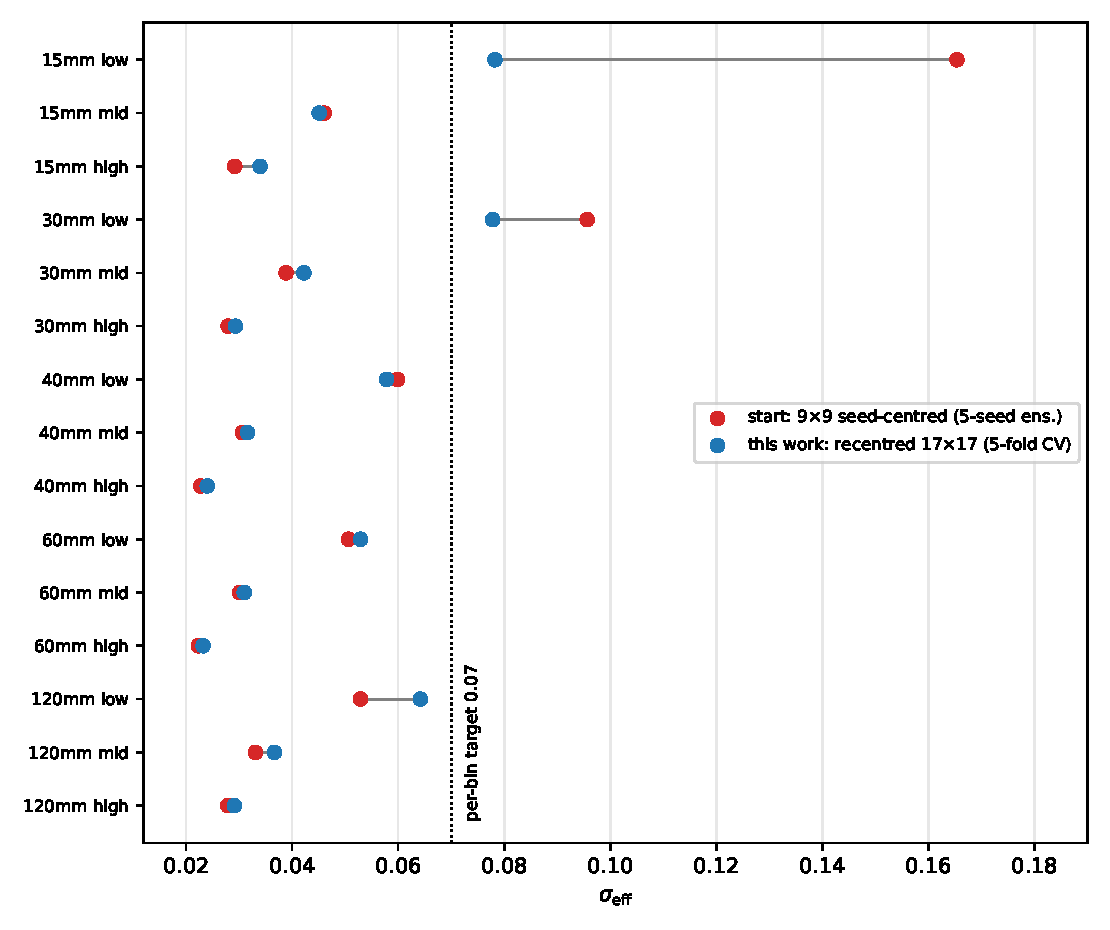
\includegraphics[width=0.72\textwidth]{figs/perbin_improvement.pdf}
\caption{All fifteen region--energy bins: starting configuration (red,
fixed-split five-seed ensemble) versus this work (blue, cross-validated
ensemble). The two protocols differ slightly (Section~\ref{sec:data});
the dominant moves --- 15\,mm low $0.165\to0.078$, 30\,mm low
$0.096\to0.078$ --- dwarf that difference.}
\label{fig:perbin}
\end{figure}

\begin{figure}[t]
\centering
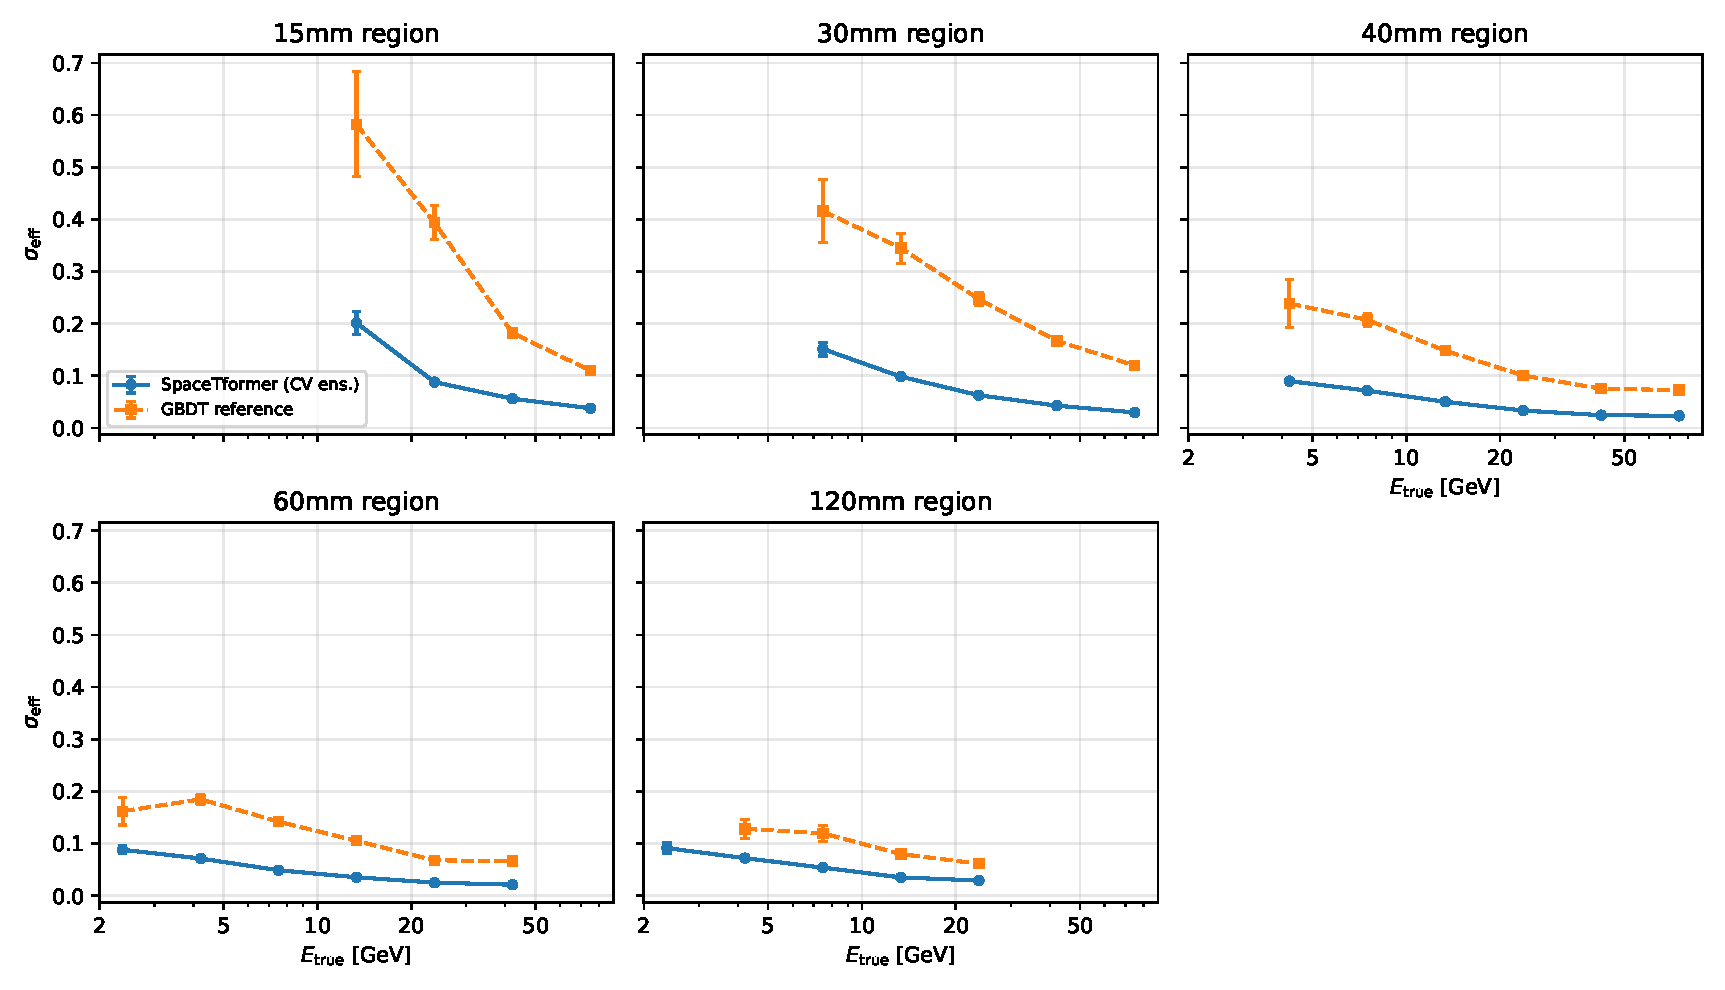
\includegraphics[width=\textwidth]{figs/resolution_vs_e.pdf}
\caption{\seff{} versus true photon energy per region: SpaceTformer
(cross-validated ensemble, circles) against the six-feature GBDT reference
(single model, fixed split, squares). Error bars are bootstrap errors over
test events. The gain is largest at low energy and in the inner regions,
matching the pileup-contamination pattern.}
\label{fig:resve}
\end{figure}

Figure~\ref{fig:resfit} fits the standard calorimeter parameterisation
$\seff(E) = a/\sqrt{E} \oplus b/E \oplus c$ to the cross-validated points
per region. The fit summarises the physics compactly: the $1/E$ term ---
which for a pileup-dominated sample plays the role of the noise term, an
energy-independent contamination in GeV --- is largest by far in the 15\,mm
region ($b = 2.1$\,GeV against $0.16$--$0.34$\,GeV in the outer regions),
while the constant terms sit below $2.5\%$ everywhere. The residual low-energy
weakness of the inner regions is pileup energy, not sampling statistics.

\begin{figure}[t]
\centering
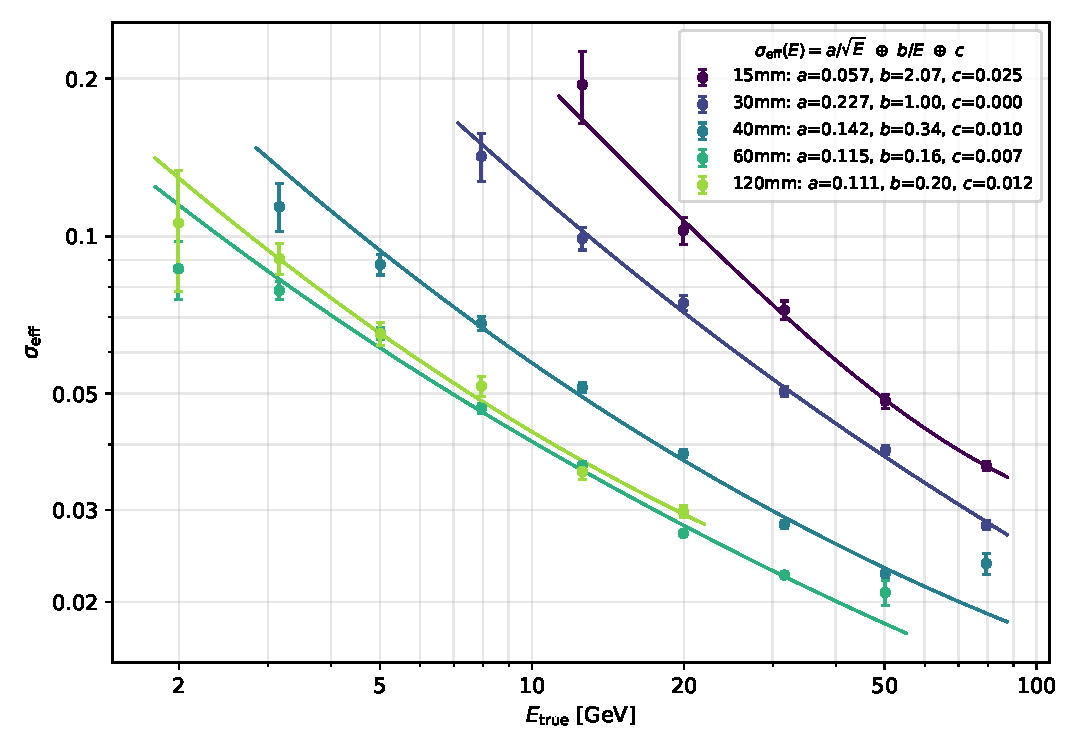
\includegraphics[width=0.72\textwidth]{figs/resolution_fit.pdf}
\caption{\seff{} versus true energy per region (cross-validated ensemble,
bootstrap errors) with the standard parameterisation
$\seff(E)=a/\sqrt{E}\oplus b/E \oplus c$ fitted per region. The $b$ (noise)
term absorbs the energy-independent pileup contamination and is an order of
magnitude larger in the 15\,mm region than in the outer ones.}
\label{fig:resfit}
\end{figure}

\begin{figure}[t]
\centering
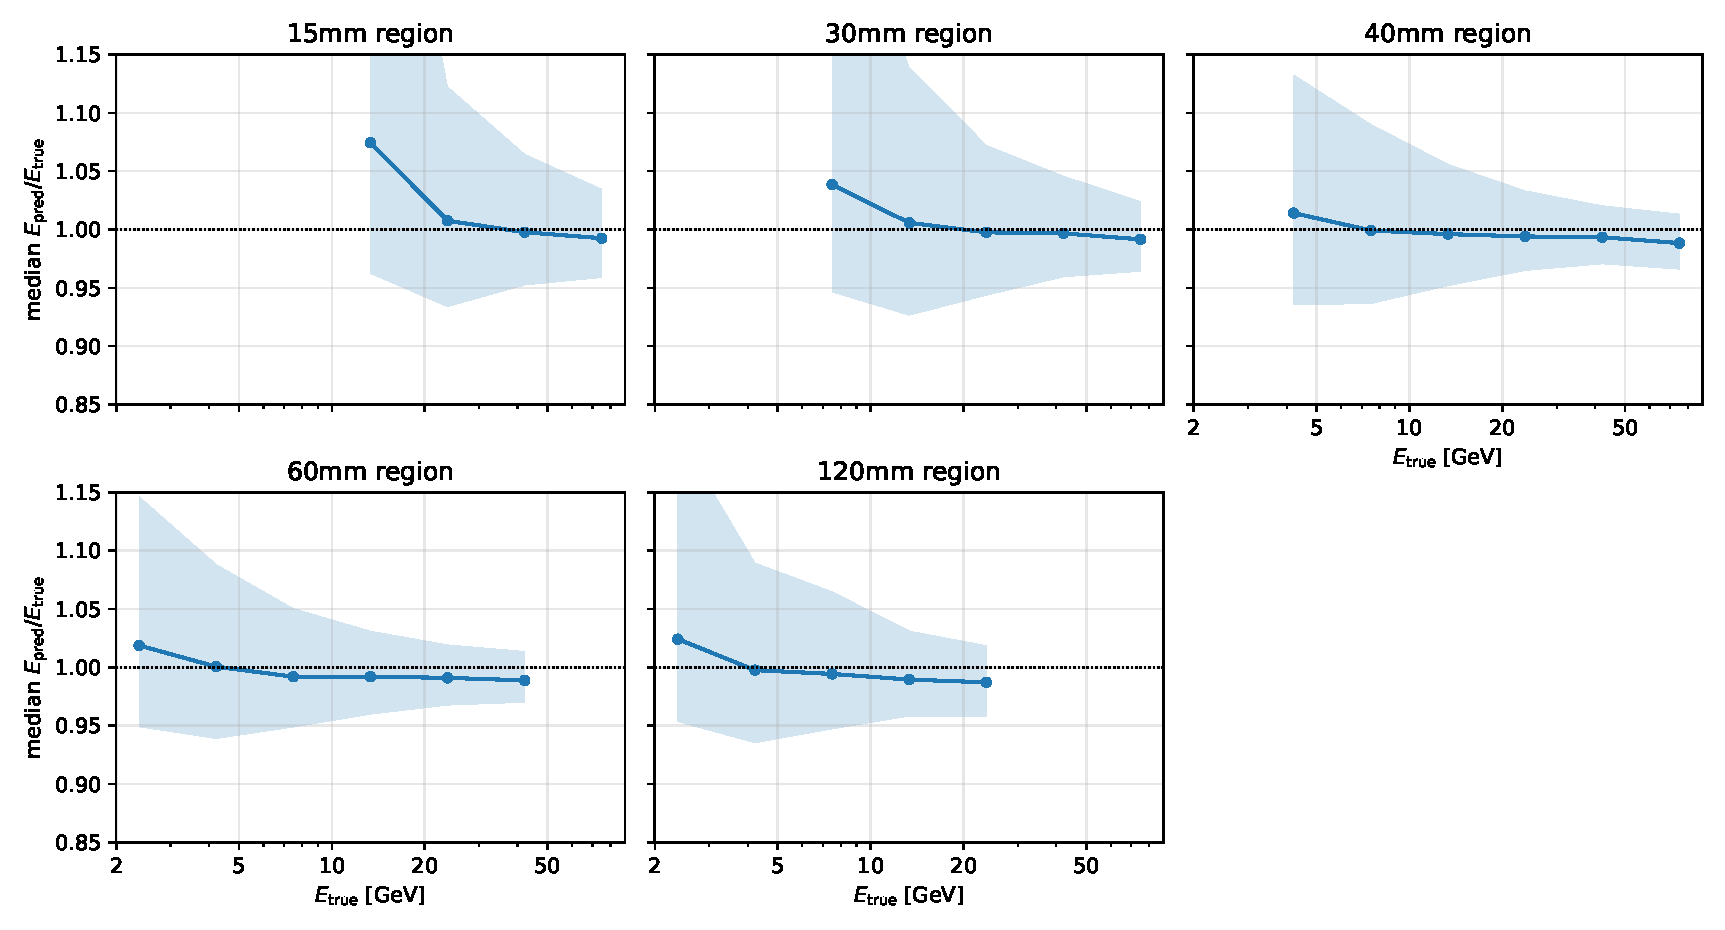
\includegraphics[width=\textwidth]{figs/linearity.pdf}
\caption{Response linearity: median $E_{\mathrm{pred}}/E_{\mathrm{true}}$
versus true energy per region for the cross-validated ensemble, with the
16--84\% band shaded. \seff{} is bias-blind, so this plot carries the scale
information the resolution table cannot.}
\label{fig:linearity}
\end{figure}

\begin{figure}[t]
\centering
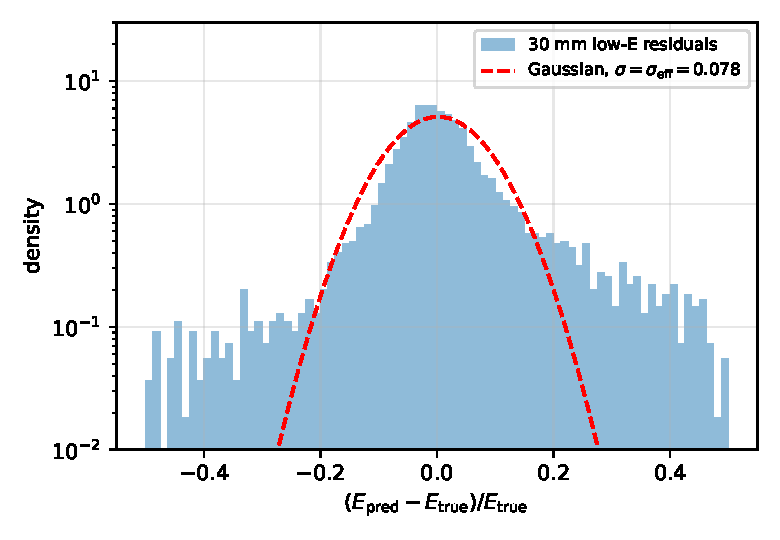
\includegraphics[width=0.55\textwidth]{figs/residuals_30mm_low.pdf}
\caption{Relative residual distribution in the 30\,mm low-energy bin
(cross-validated ensemble, log scale) against a Gaussian of width \seff.
The non-Gaussian tails are why \seff{} is the figure of merit and why
tail-reshaping interventions do not move it.}
\label{fig:residuals}
\end{figure}

\subsection{Origin of the improvement: window containment and centring}
\label{sec:gain}

The improvement over the starting configuration came from two
reconstruction-level corrections, and this subsection presents the
measurements that found them, in the order they happened.
Figure~\ref{fig:regions} first shows why the difficulty is not shared
equally across the calorimeter.

\begin{figure}[t]
\centering
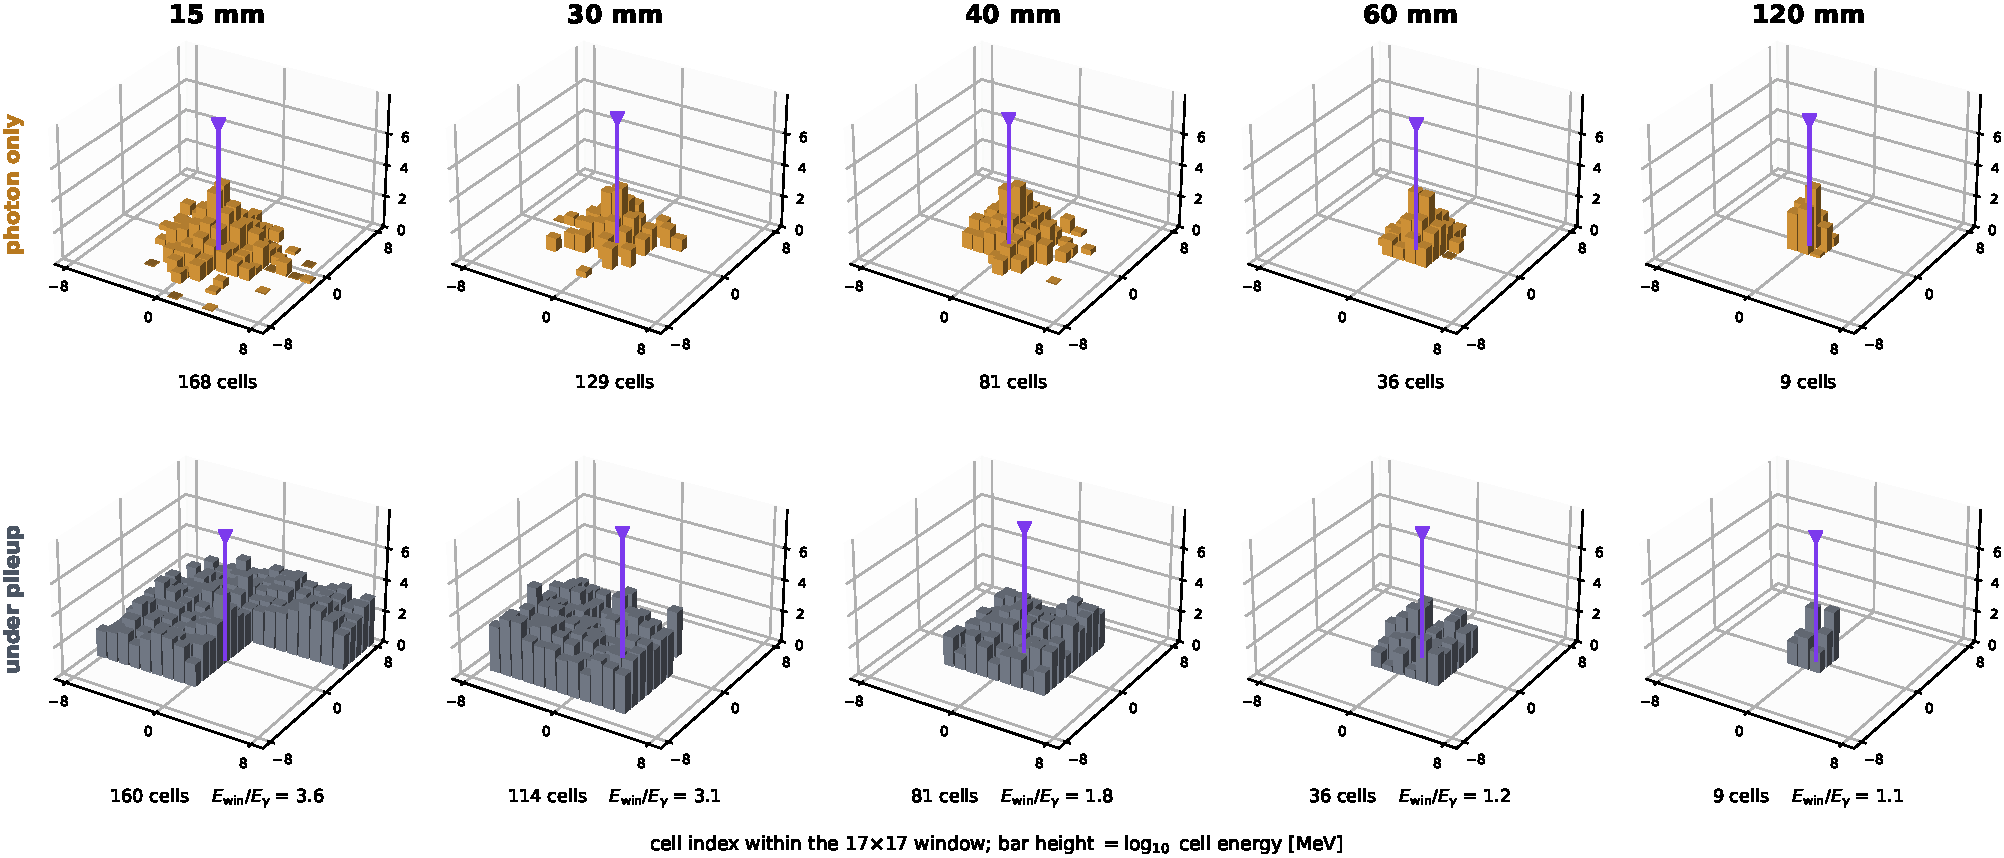
\includegraphics[width=\textwidth]{figs/regions_3d.pdf}
\caption{Why the inner regions are the hard ones. Each column is a cell
pitch; each panel shows one low-energy event of that region in the
$17{\times}17$ window, with the true photon entry marked. Top: the
pileup-free clean sample, so the bars are the photon alone. Bottom: the
minimum-bias sample, the same region under pileup. Annotations are medians
over the whole sample, not properties of the displayed event. The photon
itself is compact everywhere --- $94$--$100\%$ of its energy falls within
$3{\times}3$ cells of the seed on the clean sample --- so what changes
across regions is the \emph{load}: the window collects $3.6\times$ the
photon's energy at 15\,mm and $1.1\times$ at 120\,mm, spread over $160$
against $9$ fired cells. At 15 and 30\,mm the estimator therefore has to
subtract about three quarters of what it is given, and at low photon energy
that subtraction is the whole measurement.}
\label{fig:regions}
\end{figure}

The window half-width had been fixed at $w{=}4$ ($9{\times}9$ cells) from
the start of the project and never varied. Figure~\ref{fig:containment}
shows the measurement that broke this: the mean contained fraction of
\emph{cluster} energy versus window half-width, per region. At $w{=}4$ the
seed-centred window holds $41\%$ of the 15\,mm cluster's energy against
$\geq 92\%$ in the three outer regions --- one shared window width had been
silently tuned for the abundant outer regions.

Reading that figure as photon containment would be a mistake, and
separating the two is what explains the size of the gain. The cluster is
photon plus pileup. The \emph{photon} on its own is compact: measured on
the pileup-free clean sample with the window on the seed cell, its median
contained fraction is $94.4\%$ at $w{=}1$ and $99.8\%$ at $w{=}4$ in the
15\,mm region, and at least that in every other region. A seed-centred
$9{\times}9$ window would already hold all of the signal.

The window is not seed-centred, though: it is placed on the reconstructed
barycentre, which pileup drags a median $3.1$ cells away from the photon at
15\,mm. Measured on the paired sample, where the photon's contribution to
each cell is known, a \emph{barycentre}-centred window at 15\,mm holds a
median $1.2\%$ of the photon at $w{=}1$, $56\%$ at $w{=}2$, $97\%$ at
$w{=}3$ and $99.6\%$ at $w{=}4$ --- and the tail matters more than the
median: the fraction of events keeping less than $90\%$ of the photon is
$73\%$, $38\%$, $7.8\%$ and $0\%$ at $w{=}2,3,4,6$. The wide window is
therefore not compensating for a wide shower. It is making the aperture
robust to an imprecise centre, and the region where the centre is worst in
cell units is exactly the region the window fixed.

Above $w{=}6$ the photon is fully contained in every event, yet the window
scan below keeps improving to $w{=}8$--$10$. That remaining part is not
coverage: the extra cells carry no signal, and what they carry is the
pileup field the estimate has to subtract --- at 15\,mm the $17{\times}17$
window holds $3.6$ times the photon's own energy, over a median of 160
fired cells (Figure~\ref{fig:regions}). Two controls separate the roles.
For a plain calibrated sum with no model, widening the window makes the
15\,mm low-energy bin monotonically \emph{worse} ($0.36 \to 0.53$ from
$w{=}1$ to $w{=}8$), so the outer cells are not signal to be added. And
restricting the network's gated sum to a central core while the encoder
still attends over the whole window costs $15\,$mm low-E $0.0863$ at
core $w{=}4$ and $0.1270$ at core $w{=}2$ against $0.0755$ for the full
sum --- tracking the truncation tail above almost exactly. That the damage
is truncation and not the core idea is confirmed by repeating it on a
window centred by the learned pointer of Section~\ref{sec:pointing}, whose
median error is $0.16$ cells: there a $w{=}2$ core scores $0.0389$, equal
to the same configuration with the full sum, where on a barycentre-centred
window it scores $0.0436$. With an accurate centre the energy sum needs 25
of the 289 cells and the rest are read but never summed --- no resolution
is gained, but the readout becomes a much smaller object than the window it
sits in. The window plays both roles, and the measurements say where each
one takes over.

\begin{figure}[t]
\centering
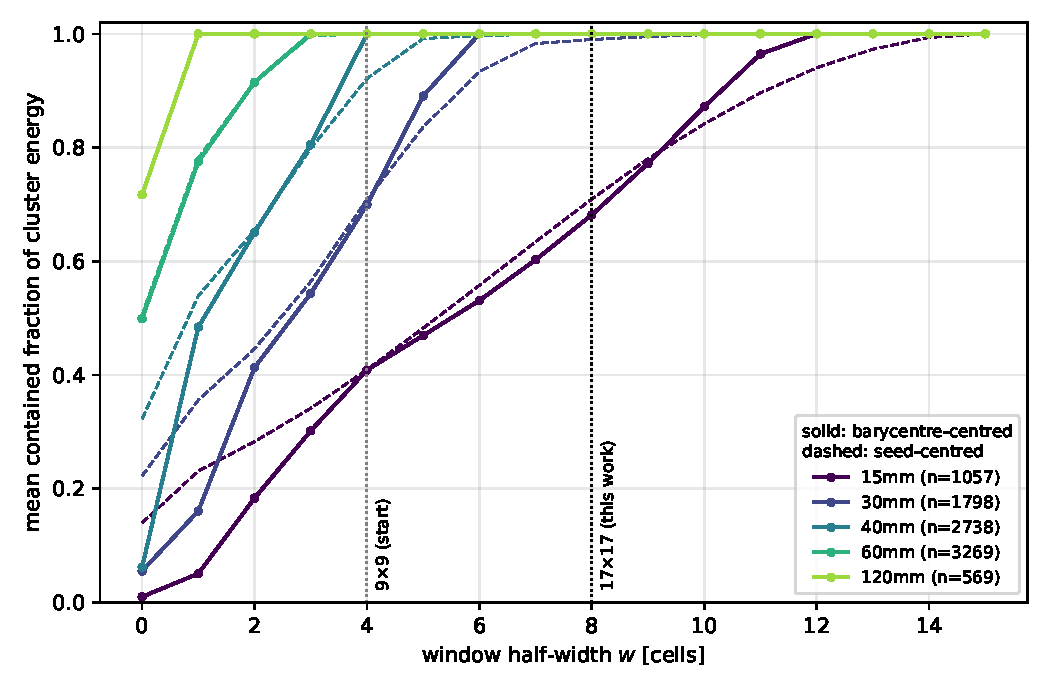
\includegraphics[width=0.68\textwidth]{figs/containment.pdf}
\caption{Mean contained fraction of cluster energy versus window half-width
$w$, per region, on the minimum-bias sample (12 files, 9{,}431 events),
for barycentre-centred (solid) and seed-centred (dashed) windows. The
vertical lines mark the starting $9{\times}9$ window and this work's
$17{\times}17$. At $w{=}4$ the 15\,mm region is the only one below half
containment.}
\label{fig:containment}
\end{figure}

Sweeping the seed-centred window from $5{\times}5$ to $21{\times}21$
(Figure~\ref{fig:windowscan}) confirms the diagnosis in resolution space:
15\,mm low-E falls from $0.186$ to $0.102$ as the window
opens --- the single largest lever found in the whole project --- while the
\emph{aggregate barely moves} ($0.038$--$0.041$ across the whole scan),
because the outer regions dominate the event count and were already
contained. That flatness is exactly how the defect stayed invisible: the
aggregate metric hid it. Ring summaries (coarse sums of the cells outside
the window, a spatial analogue of the token patching of~\cite{patchjets})
let $w{=}8$ match $w{=}10$ at half the
tokens, but only extend a resolved core; at $w{=}4$ they recover little of
what truncation destroys.

\begin{figure}[t]
\centering
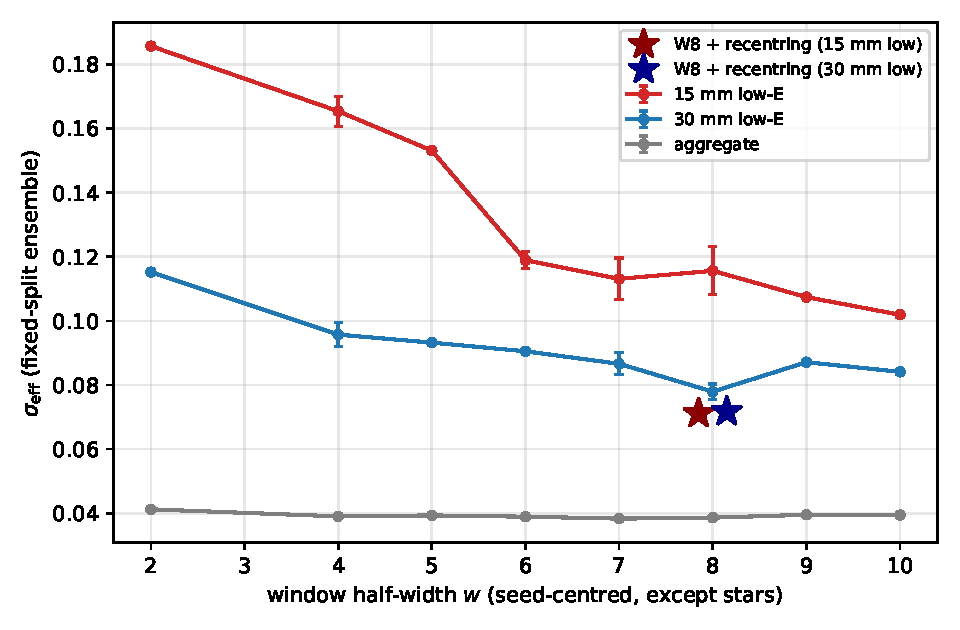
\includegraphics[width=0.66\textwidth]{figs/window_scan.pdf}
\caption{The window scan: \seff{} versus window half-width, seed-centred
(circles; fixed-split ensembles, error bars where multi-seed), with the
recentred $w{=}8$ configuration as stars. The aggregate is flat while the
worst bin halves: the aggregate metric hid the defect.}
\label{fig:windowscan}
\end{figure}

The second correction is \emph{where} the window sits. Re-centring it on
the cluster energy barycentre gives the biggest single step in the
cumulative decomposition (Table~\ref{tab:gain}: $0.1156 \to 0.0711$), and
it invites a wrong reading --- that the barycentre localises the photon better
than the seed cell. That reading is measurably false.
Figure~\ref{fig:misseed} shows the distance of each candidate centre from
the true photon entry point in the 15\,mm region: the seed cell is
\emph{much closer} to the photon (median $0.44$ cells against $3.06$), yet
the barycentre-centred window performs better. The window is not a photon-pointer; it
is an aperture, and what matters (Figure~\ref{fig:containment}, solid vs
dashed) is that the aperture covers the energy field --- photon tail plus
the pileup the model must subtract --- and gives the network a coordinate
frame anchored to that field rather than to one volatile cell. (The
decomposition in Table~\ref{tab:gain} ends at the cross-validated
$0.0783$.) Centre
estimators aimed at better photon localisation (an argmax-iterated
log-centroid, a hybrid that follows the seed except on disagreement, a
clustered $3{\times}3$ seed) were all measured worse than the plain
barycentre.

\begin{table}[h]
\centering
\caption{Cumulative decomposition of \seff{} in the 15\,mm low-energy bin.
The first three rows use the development protocol (fixed split, five-seed
ensemble); the last row is the out-of-sample cross-validated number, higher
because its per-fold ensembles are smaller --- the two protocols are not
directly comparable and both are shown deliberately.}
\label{tab:gain}
\begin{tabular}{lcll}
\toprule
step & 15\,mm low-E & protocol & mechanism\\
\midrule
$9{\times}9$ seed-centred window & 0.1654 & fixed split & centre error truncates signal\\
widen to $17{\times}17$ & 0.1156 & fixed split & robust aperture + pileup context\\
+ re-centre on barycentre & 0.0711 & fixed split & smaller centre error (see text)\\
cross-validated ensemble & 0.0783(22) & CV & primary protocol\\
\bottomrule
\end{tabular}
\end{table}

\begin{figure}[t]
\centering
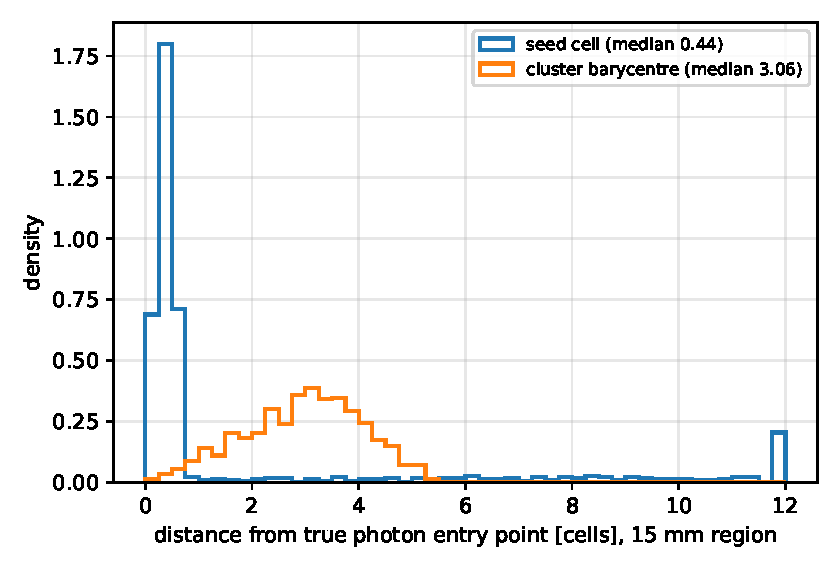
\includegraphics[width=0.55\textwidth]{figs/misseed_15mm.pdf}
\caption{Distance of the two window-centre candidates from the true photon
entry point, 15\,mm region. The seed cell is the better photon locator by
$7\times$ in the median, yet centring on the barycentre gives the better
resolution. The seed points at the photon but is wrong catastrophically in
the tail (p90 $= 8.3$ cells), while the barycentre is wrong by a few cells
almost always; with a window wide enough to absorb a few cells of error,
the estimator that never fails badly is the better centre.}
\label{fig:misseed}
\end{figure}

\subsection{A learned two-stage window}
\label{sec:pointing}

The centring analysis leaves an open question: the barycentre-centred
window gains through error-tolerant coverage while the seed is the better locator
(Figure~\ref{fig:misseed}) --- what would a window centred on the
\emph{true} photon entry add? Retraining the final configuration with the
window centred on the true entry point (a diagnostic bound: truth is not
available at inference) gives a single-member aggregate of $0.0383$
against the five-seed member mean $0.0399 \pm 0.0005$, with the weak bins
improving by $\sim$$10\%$ --- perfect centring is worth $4\%$ aggregate,
and it is the largest in-data margin any single mechanism measurement
left on the table.

That bound is reachable because the network can point. The auxiliary
position head (a three-unit regression of the photon's seed-relative
offset and time, trained alongside the quantiles at weight $0.2$) turns
out to localise the photon with a median error of $0.164$ cells and a
90th percentile of $0.389$ cells over the full sample --- against the
seed's $0.43$-cell median with its $8.5$-cell 90th percentile tail at
15\,mm, and the barycentre's $3.1$-cell median drag. On its own, adding
this head already helps the energy: ten retrained members average
$0.0395 \pm 0.0004$ and their ensemble reaches $0.0380$ (paired
bootstrap against the reference ensemble: $-0.0008 \pm 0.0003$, better in
$400/400$ resamples; the first five members alone give $0.0382$).

The two-stage architecture closes the loop: a first pass points at the
photon, the window is re-cut around the pointed position, and a second
pass regresses the energy from the re-pointed window --- the
learn-where-to-look-then-measure pattern of spatial transformer
networks~\cite{stn} and deformable attention~\cite{deformabledetr},
applied to a domain where every production reconstruction uses a fixed
seed- or barycentre-centred window. Measured offline (pointer
predictions from the trained auxiliary members; the test split is
pointed by models that never saw it), the five retrained members land at
$0.0389 \pm 0.0002$ --- the five best single members of the
$134$-configuration campaign.

\begin{table}[h]
\centering
\caption{The pointing ladder. All rows use the development protocol --- the
fixed $70/15/15$ split, seed-ensembled by per-event median --- and paired
bootstrap over 400 shared resamples against the reference ensemble. The
reference row happens to read $0.0388$ here as well, numerically equal to the
cross-validated primary result of Section~\ref{sec:primary} by coincidence:
the two are computed on different event sets under different protocols and
must not be compared with each other. Only differences \emph{within} this
table are meaningful.}
\label{tab:pointing}
\begin{tabular}{lccc}
\toprule
ensemble & members & aggregate \seff{} & paired $\Delta$ vs reference\\
\midrule
reference (recentred window) & 5 & 0.0388 & ---\\
+ position head & 10 & 0.0380 & $-0.0008 \pm 0.0003$, $P{=}1.00$\\
two-stage (point, re-cut, measure) & 5 & 0.0378 & $-0.0010 \pm 0.0003$, $P{=}1.00$\\
pooled across the three families & 25 & 0.0375 & $-0.0013 \pm 0.0002$, $P{=}1.00$\\
\bottomrule
\end{tabular}
\end{table}

Table~\ref{tab:pointing} gives the ensembles. The gain concentrates
exactly where the centring analysis said it would: 15\,mm low-E
$0.0670$ against the reference ensemble's $0.0711$ and 30\,mm low-E $0.0675$
against $0.0717$ ($-6\%$ each). The true-entry configuration is not a
like-for-like comparison at bin level --- it was measured with a single
member, not an ensemble --- so it bounds the aggregate gain rather than the
per-bin one. The one regression is the outermost region (120\,mm low-E
$0.0581$ vs $0.0555$), consistent with the earlier region-restricted
recentring measurement: where occupancy is low the seed already is the
photon, and re-pointing only adds noise --- the pointer should be applied
in the inner regions only. Distilling the five-seed ensemble into a
single member is a second route to the same margin ($0.0383$ ensemble,
$P{=}0.98$; a distilled single member matches the ensemble's accuracy
class at one fifth of its inference cost, which matters for the trigger
budget of Section~\ref{sec:cost}). The two routes do not stack
($-0.0003$, $P{=}0.73$ between them): both recover the same
centring-and-averaging margin, one structurally and one by imitation.

\paragraph{The gain does not survive cross-validation.} Every value above
is a development-protocol number, and we ran the obvious check: repeat the
construction inside the ten-fold protocol, training the position head on
each fold and building that fold's pointer from it, so nothing about the
photon position leaks into the fold's test events. Three folds were
completed before the run was stopped. The pointer is unaffected --- its
median error is $0.174$ cells per fold against $0.164$ on the development
split --- but the energy gain is not there. Scored on identical events, the
two-stage member reads $0.0388$ and $0.0387$ on folds 0 and 1 against the
auxiliary-head member's $0.0383$ and $0.0385$; pooling the three
cross-validated families reaches $0.0378$ where the primary recipe reads
$0.0381$ on the same events, a $0.8\%$ difference rather than the $2.6\%$
the development split showed.

We report this rather than quietly keeping the favourable protocol. The
development-split measurement is correct as made --- five members, a paired
bootstrap better in $400/400$ resamples --- and it does not transfer. The
most likely reading is that the fixed split's test set is both smaller and
easier than the full sample, so a mechanism worth a genuine but small
margin can look larger there than it is. The auxiliary position head, by
contrast, is worth about $1\%$ under both protocols, which is the level at
which we would now describe both mechanisms. The centring bound of $4\%$
stands; what is uncertain is how much of it any estimator can actually
take.

\subsection{Decomposition of the remaining error}
\label{sec:anatomy}

With the window fixed, we dissected what is left, joining per-event truth
diagnostics to the best ensemble's residuals (5{,}372 joined events;
diagnostics are truth-based and used only for analysis, never as inputs).
Four measurements structure the remainder.

\textbf{(1) The core width is pileup magnitude, not a missing mechanism.}
Splitting each weak bin at the median of the ratio of window energy to true
energy --- a direct measure of how much non-photon energy the window holds
--- separates two populations (Table~\ref{tab:anatomy}). Every low-energy
bin tested, including 120\,mm which was never window-limited or mis-seeded,
is a mixture of a clean population already at $0.04$--$0.07$ and a
pileup-heavy population near $0.10$. The inputs that describe pileup
magnitude (window-to-cluster energy ratio, occupancy, density) are already
features, so the model knows which population an event belongs to and still
cannot delete the fluctuation: this is the aleatoric component, localised.
It is what motivates reading the residual as a statistics problem
(Section~\ref{sec:scaling}) rather than a modelling one.

\begin{table}[h]
\centering
\caption{\seff{} of each low-energy bin split at the median per-event pileup
contamination (truth-based diagnostic). The pileup-heavy half sits near
$0.10$ in every region --- including 120\,mm, which never had a window or
centring problem.}
\label{tab:anatomy}
\begin{tabular}{lcc}
\toprule
bin & cleaner half & pileup-heavy half\\
\midrule
15\,mm low-E & 0.0683 & 0.0895\\
30\,mm low-E & 0.0598 & 0.0977\\
120\,mm low-E & 0.0370 & 0.0977\\
\bottomrule
\end{tabular}
\end{table}

\textbf{(2) The tails are catastrophic and separate from the core.} The
ratio of the $95\%$ to the $68\%$ residual quantile is $\approx 5$ in all
three bins of Table~\ref{tab:anatomy}, against $2.0$ for a Gaussian: a
$5$--$10\%$ population with $|$res$| \sim 0.4$--$0.6$ sits far outside the
core (Figure~\ref{fig:residuals}). \seff{} barely sees these events, so no
tail-directed intervention moves the aggregate number --- but they matter
for physics use, and their likely origin (wrong-photon matches, windows
dominated by an overlapping cluster) is a reconstruction question upstream
of regression. For deployment, the model already carries a per-event
confidence: the predicted inter-quantile width used by the calibration
(Section~\ref{sec:methods}) widens on exactly these events and can flag
them at inference without any additional head.

\textbf{(3) Ambiguity is measured, priced in, and still costs.} After
recentring, 30\,mm low-E events where the barycentre and the seed cell
agree within one cell resolve at $0.0489$; the rest at $0.0796$. The
disagreement magnitude is observable at inference and is already an input
--- the model knows which events are ambiguous and the gap persists, which
again says magnitude of ambiguity, not missing information.

\textbf{(4) Timing availability correlates the right way.} Events with more
time-stamped cells do better (15\,mm low-E: $0.0706$ with above-median
timing coverage vs $0.0823$ below), consistent with the timing ablation
(Section~\ref{sec:timing}) --- denser timing coverage in the detector
design would feed this model directly.

\subsection{What limits the measurement}
\label{sec:ceiling}

The four measurements above say what the residual is made of. This subsection
prices it: how much of the aggregate each part carries, how much of each part
any estimator could remove, and what is therefore left. All values here use the
development protocol on the pooled 31-member ensemble ($0.0376$ aggregate,
10{,}877 events), because it is the largest set of members we have; the
conclusions are ratios and carry over.

\paragraph{Where the aggregate comes from.} Table~\ref{tab:budget} gives, per
region--energy bin, its share of the sample and what the aggregate would become
if that bin were predicted perfectly. The bins with the worst resolution are
not the ones that matter most: 15\,mm low-E is $3.8\%$ of the sample and worth
$0.0022$ on the aggregate, while 60\,mm low-E is $11.3\%$ and worth $0.0057$.
Every window, centring and pointing measurement in this paper was developed
against the inner regions; the aggregate is carried by the middle ones.

\begin{table}[h]
\centering
\caption{Error budget by bin, development protocol. ``Aggregate if perfect''
replaces that bin's residuals with zero and rescores everything; it is an upper
bound on what any improvement to that bin can buy. ``Sampling part'' is
$a/\sqrt{E}$ from a per-region fit of $\sigma(E) = \sqrt{a^2/E + b^2 + c^2/E^2}$
evaluated at the bin's median energy --- the part no estimator can remove.}
\label{tab:budget}
\begin{tabular}{lccccc}
\toprule
bin & share & bin \seff{} & aggregate if perfect & sampling part & headroom\\
\midrule
60\,mm low-E & 11.3\% & 0.0513 & 0.0319 & 0.0226 & large\\
40\,mm low-E & 9.6\% & 0.0583 & 0.0321 & 0.0469 & small\\
30\,mm low-E & 6.7\% & 0.0699 & 0.0335 & 0.0513 & small\\
15\,mm low-E & 3.8\% & 0.0675 & 0.0354 & 0.0417 & moderate\\
120\,mm low-E & 2.0\% & 0.0540 & 0.0366 & 0.0291 & moderate\\
\bottomrule
\end{tabular}
\end{table}

\paragraph{Two of the three big bins are near their physics floor.} At 40\,mm
the stochastic term alone is $0.0469$ of the bin's $0.0583$, and at 30\,mm
$0.0513$ of $0.0699$: $80$ and $73$ per cent of the width is sampling
fluctuation of the shower itself, which is a property of the detector, not of
the estimator. Only 60\,mm low-E has real room --- its sampling term is
$0.0226$ against a measured $0.0513$ --- and there the dominant term is
$c/E = 0.0387$, an absolute error of $c \approx 0.29$\,GeV at that bin's
$7.5$\,GeV, which is the scale of the pileup fluctuation the window carries
($E_{\rm win}/E_\gamma = 1.25$ at 60\,mm). We tested the obvious handle: the
residual there correlates $+0.17$ with the observable window energy, but
removing a linear dependence on it, fitted on half the events and applied to
all, makes every bin $7$--$10\%$ worse. The window energy is already a global
input; the network has consumed it.

\paragraph{The variance component is exhausted.} Across 28 single members the
mean is $0.0394$ and the best $0.0386$; pooling all 31 gives $0.0376$, only
$4.7\%$ below the member mean. The median member-to-member spread on a single
event is $0.87\%$ of the prediction against a total error of $3.76\%$, so the
variance that ensembling removes is of order $(0.87/3.76)^2 \approx 5\%$ of the
budget and most of it is already gone. Members disagree with each other far
less than they disagree with the truth: the remaining error is common-mode.

\paragraph{Selection cannot help, by construction.} $8.2\%$ of events sit
beyond $3\seff$ and carry $21\%$ of the aggregate --- perfect treatment of them
alone would give $0.0296$. The model flags them (AUC~$0.93$ from its own
predicted width), but \emph{removing} them does not narrow \seff{}: cutting to
$80\%$ efficiency on a width threshold fitted per region and validation-energy
decile takes the aggregate from $0.0383$ to $0.0412$. \seff{} is the minimal
$68.3\%$ interval, and the flagged tails already lie outside it. Width-based
flags are useful for analysis-level purity; they cannot improve a quoted
resolution.

\paragraph{Two upper bounds are closed.} A window centred on the true photon
entry --- unavailable at inference, measured as a diagnostic --- is worth $4\%$
on the aggregate, and the learned pointer takes most of it on the development
split. A per-cell gate given truth is worth $10$--$12\%$ more than one fitted
from observables, and four supervision protocols failed to move the network
toward it because the information is already reaching the answer by another
route. Both of the mechanisms that a reader would propose first are therefore
bounded, and the bounds are small.

\paragraph{What is left.} Adding the pieces: the sampling floors of the two
most populous weak bins are fixed by the calorimeter; the variance component is
$5\%$ of the budget and largely removed; selection is a null by construction;
and the two structural bounds are worth a few per cent between them, most of it
taken. Within this sample we estimate the reachable floor at
$\seff \approx 0.038$, against the $0.0388$ reported. The one lever measured to
be worth more than a few per cent is the training-set size
(Section~\ref{sec:scaling}), which is not a modelling choice at all.

\subsection{Comparison of encoder architectures}
\label{sec:encoders}

The architecture campaign consumed the most compute and produced the
cleanest null. Ten alternatives to the plain transformer were measured
behind the same readout, loss and splits; several are re-implementations of
published architectures and several were our own designs, built on physics
arguments we found convincing at the time. None won.

The sharpest comparison is the paired one (Table~\ref{tab:h2h}):
ParticleNet (EdgeConv with dynamic $k$NN) and GravNet re-implemented behind
the identical readout, loss, splits and window, so the encoder is the only
difference, with two seeds per baseline and five for the transformer.
SpaceTformer performs best in every cell at every seed. One caveat is
required for fairness:
the baselines inherit our frozen training recipe, which was validated on
the transformer; they received their published architectural defaults but
no dedicated hyperparameter sweep, and the comparison should be read with
that asymmetry in mind. A dedicated six-arm sweep (learning rate halved and
doubled, and neighbourhood size $k$ raised to 24, per baseline) closes this
caveat, and we report it in full: every tuned arm still trails. ParticleNet
reads $0.0456 / 0.0408 / 0.0422$ (lr $10^{-4}$ / lr $6\times10^{-4}$ /
$k{=}24$) and GravNet $0.0443 / 0.0455 / 0.0427$. The best of the six,
ParticleNet at lr $6\times10^{-4}$, narrows the aggregate gap to $+0.0009$
(about twice the transformer's seed spread) and reaches $0.0785$ at 15\,mm
low-E (within the transformer's spread there) --- but remains $+0.0045$
behind at 30\,mm low-E, five times the spread, at $3.6\times$ the training
cost. The robust statement is therefore: no tuned baseline matches the
transformer at equal cost, and none matches it in the 30\,mm weak bin at
any cost we measured. The aggregate gaps of the paired default comparison
($+0.0016$ ParticleNet,
$+0.0038$ GravNet against the transformer's five-seed mean $0.0399$) exceed
the transformer's own seed spread of $0.0005$; the weak-bin gaps are larger
still and consistent across bins, baselines and seeds.

\begin{table}[h]
\centering
\caption{Head-to-head \seff{} under an identical fixed-split protocol.
Single models, no ensembling, which is why the transformer row differs from
Table~\ref{tab:primary}'s ensemble numbers; mean $\pm$ spread across seeds
(five for SpaceTformer, two for each baseline). Training time is per model
on one A100.}
\label{tab:h2h}
\small
\setlength{\tabcolsep}{4.5pt}
\begin{tabular}{lcccc}
\toprule
encoder & aggregate & 15\,mm low-E & 30\,mm low-E & time\\
\midrule
SpaceTformer (ours) & $\mathbf{0.0399 \pm 0.0005}$ & $\mathbf{0.0759 \pm 0.0058}$ & $\mathbf{0.0768 \pm 0.0009}$ & 33\,min\\
ParticleNet & $0.0415 \pm 0.0004$ & $0.0815 \pm 0.0003$ & $0.0872 \pm 0.0053$ & 120\,min\\
GravNet & $0.0437 \pm 0.0006$ & $0.0861 \pm 0.0045$ & $0.0922 \pm 0.0040$ & 60\,min\\
\bottomrule
\end{tabular}
\end{table}

Table~\ref{tab:encoders} is the full campaign. ``Era'' matters: early arms
ran before the window and recentring fixes, against the matching reference
of their time.

\begin{table}[h]
\centering
\caption{All encoder families measured, fixed-split protocol, aggregate
\seff{} with the era's matching transformer reference; single-seed values,
which is why the ParticleNet/GravNet rows differ slightly from
Table~\ref{tab:h2h}'s two-seed means. The two time-factorised arms are one
family measured in two eras. Screening = cut before a five-seed run.}
\label{tab:encoders}
\small
\setlength{\tabcolsep}{4pt}
\begin{tabular}{llccl}
\toprule
encoder & lineage & aggregate & reference & outcome\\
\midrule
pair transformer & pairwise tokens & 0.0627 & 0.039--0.041 & lost, early era\\
energy-flow network & Deep Sets / EFN~\cite{efn} & 0.0623 & 0.039--0.041 & lost, early era\\
spacetime-factorised (v1) & TimeSformer~\cite{timesformer} & 0.0543 & 0.039--0.041 & lost, early era\\
geometric pairwise-bias & ParT~\cite{part} & 0.0420 & 0.0390 & lost\\
grid CNN & dense image & 0.0476 & 0.039--0.040 & lost (2 seeds)\\
ConvNeXt token mixer & modern CNN & --- & --- & cut at screening\\
patch tokens (ViT-style) & spatial patching, cf.~\cite{patchjets} & --- & --- & cut at screening\\
time-sliced attention (v2) & TimeSformer, on final config & 0.0442 & 0.0402 & lost\\
GravNet & \cite{gravnet} & 0.0432 & 0.0402 & lost, paired\\
ParticleNet & \cite{particlenet} & 0.0412 & 0.0402 & lost, paired\\
masked MLP-Mixer & \cite{mixer} & 0.0654 & 0.0402 & lost\\
\midrule
token transformer & \cite{vaswani} & \textbf{0.0390} & & best encoder\\
\bottomrule
\end{tabular}
\end{table}

Three failures are informative enough to deserve a sentence each. The
\emph{time-sliced attention} arm was our own flagship design --- bucket
cells by time pull, attend within buckets, exchange pooled summaries ---
built on the observation that pileup energy has a $13$\,ns time spread at
15\,mm against $1.6$\,ns for the photon. It lost twice, on two eras of the
pipeline, because slicing removes exactly the cross-time comparisons the
full-attention model uses. The \emph{grid CNN} represents the event as a
dense image; it loses $20\%$ to the token view of the same cells --- under
pileup, most of the grid is noise, and convolution must spend capacity
learning to ignore what tokenisation simply omits. The
\emph{pairwise-bias} arm imports the Particle Transformer's
physics-motivated attention bias, which helps on jets with hundreds of
particles and well-defined pairwise invariants; at 81 noisy cells it only
constrains the attention away from what the data wanted. The \emph{masked
MLP-Mixer} replaces attention with fixed learned mixing weights across
token positions; it loses $63\%$ ($0.0654$ vs $0.0402$) because under
pileup the informative cells move event by event --- exactly the situation
content-based attention handles and position-based mixing cannot. Capacity
is not the explanation for any of this. Doubling the transformer to
$d{=}256$/6 layers collapses under the frozen recipe ($0.1179$); we
diagnosed the collapse directly, and it is an optimization artefact, not
saturation: learning-rate warmup alone recovers to $0.0692$, pre-layer
normalisation~\cite{preln} to $0.0474$, and both together restore full
trainability at $0.0412$ --- which still does not beat $d{=}128$'s
$0.0402$. Halving to $d{=}64$/2 layers costs $15\%$ ($0.0463$). The
conclusion survives the diagnosis in a stronger form: the large model
\emph{trains} and still yields no gain. At 81--289 tokens per event, full
attention is not the bottleneck, and no cheaper alternative matches it.

\subsection{Interpretation of the learned gate}
\label{sec:gate}

The readout's per-cell gate looks like it should estimate the photon
fraction of each cell, yet on a paired overlay sample with per-cell truth
labels its correlation with the true fraction is only $0.211$. We measured
four ways of ``fixing'' this: direct supervision of the gate on overlay
truth, an auxiliary fraction head, per-cell prior features from a fitted
estimator, and teacher distillation from that estimator. All four are
neutral or worse. Meanwhile a gradient-boosted per-cell estimator given the
identical per-cell observables reaches correlation $0.945$ on the same
sample --- the information is present in the inputs, and the network routes
it around the gate rather than through it. The gate is a learned attention
weight inside an integral, not a physical quantity, and constraining it to
be physical costs resolution. We flag this because the ``interpretable
gate'' framing is publication-ready and, on this measurement, wrong.

The gate study sat inside a larger arc on \emph{overlay supervision}:
manufacturing per-cell truth by overlaying clean photon showers onto pileup
and training against those labels. Its structural half worked --- an
explicit subtract-then-calibrate decomposition, where one branch estimates
the pileup field and a second calibrates what remains, reached $0.0465$ as
an ensemble in its era --- but the supervision half did not: training the
subtraction branch on overlay labels was neutral against letting it learn
freely. A domain measurement explains why: synthetically overlaid events
are distinguishable from real minimum-bias events by a classifier at
AUC~$0.93$ on cell-level observables, so labels manufactured by overlaying
do not come from the distribution the model must serve. Structure helped;
manufactured labels did not.

\subsection{Timing}
\label{sec:timing}

Per-cell timing is the physics handle expected to matter under pileup, and
Figure~\ref{fig:timing} shows it is a \emph{pileup} handle specifically.
Retraining the starting configuration with both timestamps removed gives
aggregate $0.0485$ against $0.0390$, 15\,mm low-E $0.2033$ against
$0.1654$, and 30\,mm low-E $0.1556$ against $0.0957$ --- timing carries
$20\%$ of the aggregate resolution and up to $38\%$ in the weak bins ---
while the identical ablation on the pileup-free clean sample is neutral
($0.0476$ with vs $0.0460$ without). The timestamps carry no energy
information; their entire value is separating overlapping sources in time

\begin{figure}[t]
\centering
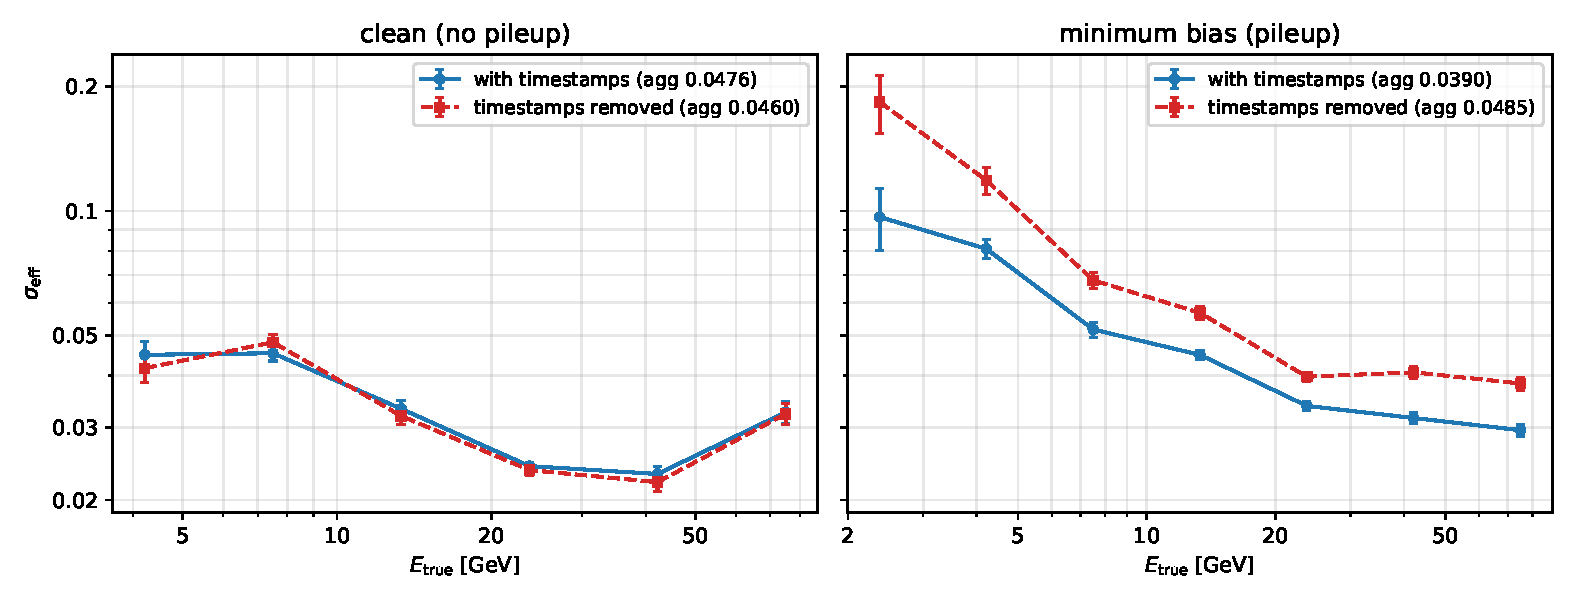
\includegraphics[width=0.94\textwidth]{figs/timing_ablation.pdf}
\caption{The timing ablation, side by side on the pileup-free clean sample
(left; two-seed ensembles, earlier-era configuration) and the minimum-bias
sample (right; the starting configuration). Removing the per-cell
timestamps is neutral without pileup and costs $20\%$ aggregate ---
concentrated at low energy --- under pileup: timing is a pileup-separation
tool, not an energy observable.}
\label{fig:timing}
\end{figure}
\todo{state the simulated timestamp resolution once confirmed from the
simulation configuration}. But every \emph{engineered} use of timing loses
to handing the network the raw timestamps: three time-pull coordinate
constructions (per-cell time scaled by its expected spread), hard timing
cuts, time-sliced attention, an inverse-variance front/back combination,
and a Fourier basis on the raw time channels ($0.0413$ vs $0.0402$) were
all measured and all reduce or at best match. The network already
extracts what the timestamps carry; pre-digesting them removes information.
The result independently supports the HL-LHC timing programme --- per-cell
timing in high-granularity calorimeters~\cite{hgcal} and dedicated timing
layers for four-dimensional vertexing~\cite{mtd}: per-cell timestamp
resolution, and the fraction of cells that carry a timestamp at all, feed a
model like this one directly.

Three interventional probes on the trained model say \emph{how} the
timestamps are read, which the retraining ablation cannot. Perturbing the
inputs of the trained final member at evaluation (recalibrating per
variant): (i)~permuting the timestamps among the cells of the same event
--- the identical multiset of values, reassigned --- degrades the
aggregate to $0.398$, \emph{worse} than zeroing them ($0.310$), so the
model reads per-cell time structure rather than any pooled event
statistic; (ii)~a rigid shift of every timestamp in an event, which
changes nothing pairwise, already costs $44\%$ at half a standard
deviation --- the model anchors on the absolute median-subtracted scale
where in-time means near zero, which together with the pairwise-bias
encoder's null (Section~\ref{sec:encoders}) closes the case for an
explicit relative-time attention mechanism; and (iii)~coarsening the
timestamps onto a grid costs $11\%$ at a quarter of the per-event time
spread and $19\%$ at half --- the network exploits timing down to roughly
a quarter of the spread the sample provides, so the simulated timestamp
resolution matters at exactly that grain.

\subsection{Negative results}
\label{sec:closed}

Table~\ref{tab:closed} is the record of measured null results beyond the encoder
campaign. Each row is a mechanism a reviewer --- or we ourselves --- would
otherwise propose. For scale: the single-member spread on the aggregate is
$0.0010$ and the bootstrap error on the ensemble aggregate is $0.0002$
(Section~\ref{sec:data}); rows marked ``worse'' exceed it, rows marked
``neutral'' sit within it.

\begin{table}[h]
\centering
\caption{Negative results, all measured under the frozen protocol.
Aggregate \seff{} comparisons are against the matching-protocol value
$0.0379$ (the half-sample CV ensemble current when each was measured) or
$0.0402$ (fixed-split single seed) as labelled.}
\label{tab:closed}
\footnotesize
\setlength{\tabcolsep}{4pt}
\begin{tabular}{@{}p{0.24\textwidth}p{0.40\textwidth}p{0.32\textwidth}@{}}
\toprule
family & protocols tried & outcome\\
\midrule
gate supervision & 4 (direct, aux head, prior feature, distill) & neutral or worse\\
engineered timing & 5 (pulls $\times$3, cuts, slices, front/back comb.) & all worse\\
training recipe & lr $\times$2, batch $\times$2, jitter $\times$2 & 0.0422--0.0462 vs 0.0402\\
ensembling & learned stacking on held-out data & 0.0414 vs 0.0379, worse\\
recalibration & post-hoc per (region $\times$ E-decile) & 0.0386 vs 0.0379, worse\\
test-time augmentation & D4 averaging & neutral, $8\times$ cost\\
capacity & $d{=}256$/6L; $d{=}64$/2L & 0.1179 / 0.0463, both worse\\
capacity, diagnosed & + warmup; + pre-LN~\cite{preln}; + both & 0.0692; 0.0474; 0.0412 --- trains, no gain\\
time representation & Fourier basis on raw time channels & 0.0413 vs 0.0402, worse\\
slot decomposition & $K{=}4$ competing readout queries & 0.0406 vs 0.0402, neutral\\
time-gated readout & multiplicative time gate on the final window & 0.0399 vs 0.0399 mean, neutral\\
train-time augmentation & D4 transforms of the window & 0.0401 vs 0.0402, neutral\\
quality selection & cut on predicted quantile width & worse at every efficiency (see text)\\
core-restricted sum & gated sum over $w{=}4$; $w{=}2$ core & 0.0404; 0.0436 vs 0.0399\\
core sum on a pointed window & $w{=}2$ core, learned centre & 0.0389, equal to full sum\\
\bottomrule
\end{tabular}
\end{table}

Two of the new rows carry lessons beyond their null. The quality-selection
row fails \emph{by construction}, not by accident: the predicted
interquartile width does flag the catastrophic events, but \seff{} is the
minimal $68.3\%$ interval --- a robust statistic --- and the flagged tails
already lie outside it, so removing them cannot narrow it (cutting to
$80\%$ efficiency \emph{worsens} the aggregate from $0.0383$ to $0.0412$;
the thresholds were fitted per region and validation-energy decile to
exclude the trivial version of the cut that simply empties the hard bins).
Width-based flags remain useful for analysis-level purity; they cannot improve the
quoted resolution. And the train-time augmentation null is a control for
the scaling claim: an eight-fold increase in geometric variety yields
nothing, while the measured curve implies that tripling the \emph{real}
sample yields $\sim$$18\%$ --- what $N^{-0.18}$ purchases is diversity of pileup
configurations, which symmetry transforms cannot manufacture. The data
request has no augmentation shortcut.

Beyond these, fourteen per-cell and global feature mechanisms were measured
on the same protocol. The ones that stayed: extra reconstruction globals,
local density, and the clean-sample auxiliary. The ones measured
neutral-or-worse, each with its row in the repository ledger: time-pull
coordinates ($+0.017$ at 15\,mm low-E), orthogonal-residual coordinates,
absolute time, local energy fraction, depth ratio, gate-side global
injection, physics/occupancy summaries, FiLM conditioning on pileup
context, signed gates ($+0.009$ at 15\,mm low-E on the recentred
configuration), trainable gate temperature, low-energy cell reweighting at
four strengths, and millimetre-unit geometry (neutral on the final
configuration; its one gain before recentring was superseded by recentring
itself). The consistent reading across all fourteen: the token set already
carries the information, and the model finds it without hand-built
coordinates.

\subsection{Computational cost}
\label{sec:cost}

A reconstruction algorithm is only deployable at a cost, so we benchmark
inference throughput on commodity hardware (laptop CPU, i9-13900HX, batch
64, median of 5 timed passes on an idle machine).
Figure~\ref{fig:throughput} places each model family on the
accuracy--throughput plane. At the $9{\times}9$ window a single transformer
runs at $\sim$5{,}000 clusters/s (0.20\,ms per cluster) and the five-seed
ensemble at 992 clusters/s; the GBDT reference is $3.3\times$ faster per
cluster than a single transformer pass and $3.1\times$ worse in resolution;
the analytic calibrated sum is effectively free ($5.6\times10^6$
clusters/s) and $4.6\times$ worse. The final $17{\times}17$ recentred
configuration pays the quadratic attention cost of $289$ vs $81$ tokens:
555 clusters/s per model, 111 clusters/s for the five-member ensemble,
measured on the same harness. On one H100 GPU the same configuration
reaches 1{,}017 clusters/s at batch 1 (latency-bound) and 41{,}345
clusters/s at batch 1024 --- $24\,\mu$s per cluster for a single model,
$121\,\mu$s for the five-member ensemble --- which brings batched
inference into the regime where a conversation about high-level-trigger
deployment becomes quantitative (\texttt{reports/benchmark\_gpu.csv}). Accuracy per compute is therefore a real
trade-off the experiment can choose along: from the free analytic sum to
the full ensemble spans four orders of magnitude in throughput for a
$4.7\times$ span in resolution.

\begin{figure}[t]
\centering
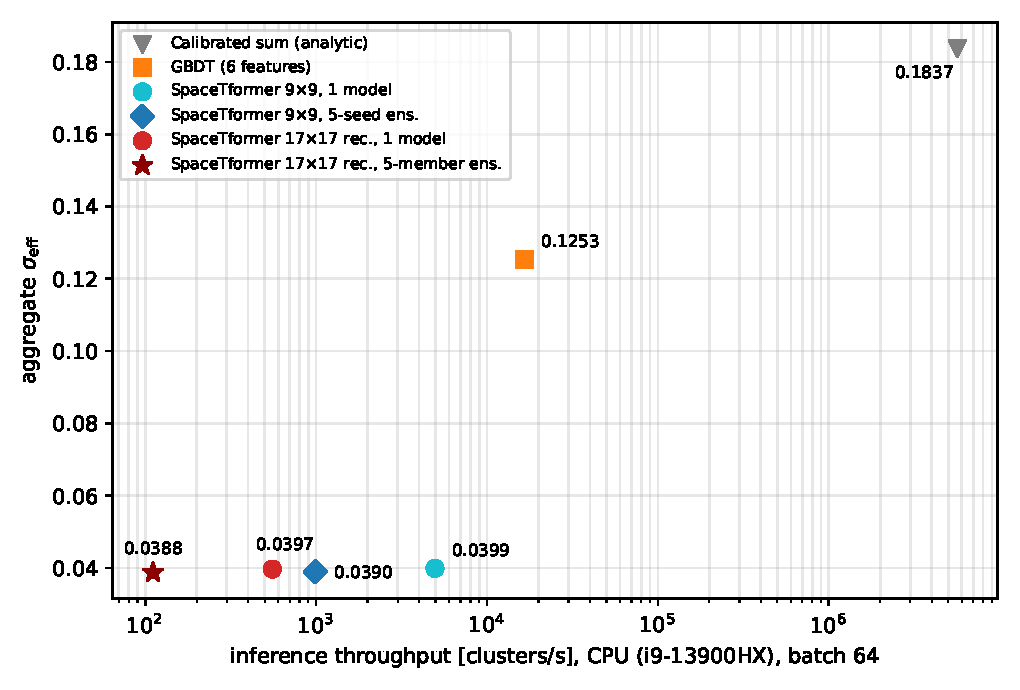
\includegraphics[width=0.62\textwidth]{figs/accuracy_vs_throughput.pdf}
\caption{Aggregate \seff{} against inference throughput (CPU, batch 64;
log scale). The four left points use the fixed-split protocol; the two
$17{\times}17$ points use the single-member mean ($0.0397$) and the
cross-validated ensemble ($0.0388$), with the forward-pass rate measured at
289 tokens on the same harness. The transformer obtains its resolution by
reading cells individually, and the window that fixed the weak bins costs a
further $9\times$ in attention compute.}
\label{fig:throughput}
\end{figure}

\subsection{Dependence on training-sample size}
\label{sec:scaling}

With representation, architecture, supervision, recipe, ensembling and
calibration each closed by measurement, the remaining open lever is
training-set size, and we measured its slope directly: the final
configuration retrained on deterministic $25\%$, $50\%$ and $75\%$
subsamples of the training set (validation and test untouched, same recipe,
three seeds per point) plus the full-data point
(Figure~\ref{fig:scaling}). The four points are strikingly linear in
log--log and give
\[
\seff \propto N^{-0.18},
\]
identically for single models ($0.0524 \to 0.0466 \to 0.0439 \to 0.0402$)
and for three-seed ensembles (exponent $-0.179$), and the worst bin scales
in parallel (15\,mm low-E: $0.1254 \to 0.0729$ across the same points).
This within-protocol curve supersedes two earlier confounded two-point
estimates ($-0.13$ and $-0.28$) and lands between them; power-law scaling
of error with dataset size is the generic empirical behaviour of deep
networks~\cite{hestness,kaplan}, so the linearity is expected even if the
exponent is task-specific. Extrapolated
threefold --- an extrapolation, and labelled as such --- it predicts an
aggregate of $\approx 0.033$. The qualitative case is independent of the
fit: every intervention that did not add training data saturated at
aggregate $\approx 0.039$, and the residual error is dominated by per-event
pileup magnitude (Section~\ref{sec:anatomy}), a statistical quantity that
more data smooths.

\begin{figure}[t]
\centering
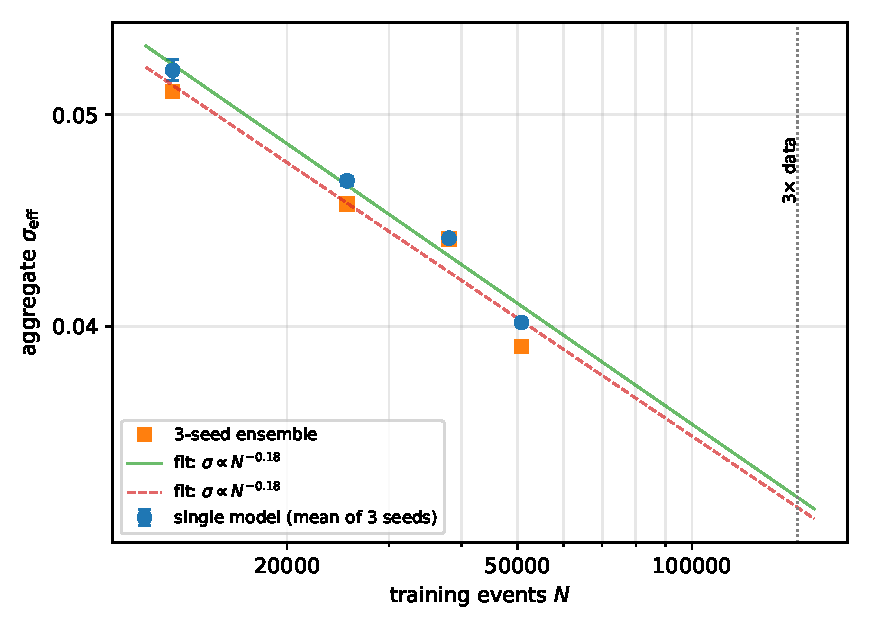
\includegraphics[width=0.6\textwidth]{figs/scaling_curve.pdf}
\caption{The measured data-scaling curve: aggregate \seff{} of the final
configuration retrained on $25/50/75/100\%$ of the training set
(fixed-split protocol, three seeds per point; the $75\%$ point completed
one seed). Both the single-model mean and the three-seed ensemble fit
$\seff \propto N^{-0.18}$; the dotted line marks a tripled sample, at a
predicted aggregate of $\approx 0.033$.}
\label{fig:scaling}
\end{figure}

\section{Limitations and future work}
\label{sec:limits}

Five limitations bound the claims. (0) The clearest one is recent: the two-stage window's development-split gain does not reproduce under cross-validation (Section~\ref{sec:pointing}), which is a warning about every development-split number in this paper. They are labelled wherever they appear, but a margin of a few per cent measured on the fixed split should be treated as a hypothesis until the ten-fold protocol confirms it. (1) Everything is measured on one
simulated sample of one detector concept; the diagnosis method transfers,
the numbers may not. Two internal transfers partially mitigate this: the
pileup-free clean sample is a second distribution on which the timing
conclusion reproduces with the opposite sign
(Figure~\ref{fig:timing}), and the window diagnosis holds across five
detector regions whose granularity spans a factor of eight --- effectively
five related sub-detectors. (2) The architecture comparison is paired and now includes a per-baseline
hyperparameter sweep (learning rate, neighbourhood size), but the sweep is
small; its conclusion is about this task's regime, not about the
architectures in general. (3) The
scaling prediction at $3\times$ data is an extrapolation beyond the
measured range of the (otherwise clean) four-point curve. (4) The half-sample preview of the
primary table read $0.0379$ aggregate; the complete ten-fold table reads
$0.0388$ --- a real lesson in why half-done cross-validation must not be
quoted as final, which we record here deliberately.

On venue fit, we state the contribution class plainly: this paper offers a
measurement-driven diagnosis, a controlled architecture comparison, and a
ledger of verified negative results --- not a new architecture; it should
be evaluated as such.

Three directions follow directly from the measurements. The catastrophic
tails (Section~\ref{sec:anatomy}) are a reconstruction problem ---
wrong-photon matches and overlapping clusters --- addressable upstream of
any regressor. The timing-coverage correlation suggests that denser
timestamp coverage is a detector-design lever this model would convert
directly into resolution. And the data request is now quantitative:
tripling the minimum-bias simulation is predicted, with stated caveats, to
bring the aggregate below $0.035$.

\section{Conclusions}

On a simulated minimum-bias PicoCal sample, SpaceTformer reaches
$\seff = 0.0388 \pm 0.0002$ aggregate, fully out-of-sample over the complete
ten-fold protocol --- a $3.2\times$ improvement over a six-feature GBDT
reference --- and beats paired re-implementations of ParticleNet and
GravNet in every measured cell at every seed, at a fraction of their cost.
The improvement over our own starting point --- $53\%$ in the worst
region--energy bin --- came entirely
from measuring and fixing the input representation: window containment and
window centring. The same diagnosis, pushed one step further, produced the
learned two-stage window of Section~\ref{sec:pointing}, which points
before it measures and takes the development-protocol ensemble to
$0.0378$; a cross-validated re-run of the same construction does not
reproduce that margin, and we report both. What does hold under either
protocol is the auxiliary position head, at about $1\%$. Everything else we tried is reported with its numbers in
Sections~\ref{sec:encoders}--\ref{sec:closed} and the scored
ledger versioned with the code, so it does not have to be re-tried silently.
Pricing the residual bin by bin (Section~\ref{sec:ceiling}) puts the reachable
floor on this sample at $\seff \approx 0.038$: the two most populous weak bins
are $73$--$80\%$ sampling fluctuation, the variance ensembling removes is $5\%$
of the budget and largely gone, selection cannot narrow a robust interval, and
the two structural bounds a reader would propose first are worth a few per cent
between them. The measured scaling curve, $\seff \propto N^{-0.18}$, therefore
makes the path below that a data request rather than an architecture search.

\section*{Acknowledgements}

This work was carried out within Google Summer of Code 2026 for the LHCb
PicoCal project. I thank my mentors in the LHCb PicoCal group for the
simulated samples, weekly guidance, and the error-analysis discipline this
paper is built on. \todo{Named acknowledgements and LHCb
publication-approval status to be settled with the mentors before any
submission; single-author use of collaboration simulation may require
Editorial Board review or release as a collaboration note.}

\section*{Code and data availability}

All experiments run from a single training script with a flag for every
mechanism in this paper; the prediction CSVs behind every reported number
and the scripts that generate every figure are versioned alongside the code
at \url{https://github.com/Lworakan/GSoC2026-picocal-spacetime-transformer}.
The simulated samples belong to the LHCb collaboration and are not
redistributed.


\begin{thebibliography}{99}
\bibitem{particlenet} H.~Qu, L.~Gouskos,
\emph{Jet tagging via particle clouds},
Phys.\ Rev.\ D 101 (2020) 056019, arXiv:1902.08570.
\bibitem{gravnet} S.~R.~Qasim, J.~Kieseler, Y.~Iiyama, M.~Pierini,
\emph{Learning representations of irregular particle-detector geometry with
distance-weighted graph networks}, Eur.\ Phys.\ J.\ C 79 (2019) 608,
arXiv:1902.07987.
\bibitem{vaswani} A.~Vaswani et al.,
\emph{Attention Is All You Need}, NeurIPS 2017, arXiv:1706.03762.
\bibitem{part} H.~Qu, C.~Li, S.~Qian,
\emph{Particle Transformer for Jet Tagging}, ICML 2022, arXiv:2202.03772.
\bibitem{timesformer} G.~Bertasius, H.~Wang, L.~Torresani,
\emph{Is Space-Time Attention All You Need for Video Understanding?},
ICML 2021, arXiv:2102.05095.
\bibitem{patchjets} A.~Wang, Z.~Zhao, A.~Xia, C.~Sun, A.~Gandrakota,
J.~Ngadiuba, R.~Cavanaugh, J.~Duarte,
\emph{Patch Hierarchical Attention Transformer for Efficient Particle Jet
Tagging}, arXiv:2605.21789 (2026).
\bibitem{clustex} Y.~Maidannyk, F.~Couderc, J.~Malcl\`es, M.~\"O.~Sahin,
\emph{Reconstruction of overlapping electromagnetic showers in calorimeters
using Transformers}, Eur.\ Phys.\ J.\ C 86 (2026) 873, arXiv:2603.18172.
\bibitem{deepsets} M.~Zaheer et al.,
\emph{Deep Sets}, NeurIPS 2017, arXiv:1703.06114.
\bibitem{efn} P.~T.~Komiske, E.~M.~Metodiev, J.~Thaler,
\emph{Energy Flow Networks: Deep Sets for Particle Jets},
JHEP 01 (2019) 121, arXiv:1810.05165.
\bibitem{mixer} I.~Tolstikhin et al.,
\emph{MLP-Mixer: An all-MLP Architecture for Vision}, NeurIPS 2021,
arXiv:2105.01601.
\bibitem{mamba} A.~Gu, T.~Dao,
\emph{Mamba: Linear-Time Sequence Modeling with Selective State Spaces},
COLM 2024, arXiv:2312.00752.
\bibitem{dinov3} O.~Sim\'{e}oni et al.,
\emph{DINOv3}, arXiv:2508.10104 (2025).
\bibitem{xgboost} T.~Chen, C.~Guestrin,
\emph{XGBoost: A Scalable Tree Boosting System}, KDD 2016, arXiv:1603.02754.
\bibitem{lightgbm} G.~Ke et al.,
\emph{LightGBM: A Highly Efficient Gradient Boosting Decision Tree},
NeurIPS 2017.
\bibitem{hgcal} CMS Collaboration,
\emph{The Phase-2 Upgrade of the CMS Endcap Calorimeter},
CERN-LHCC-2017-023, CMS-TDR-019 (2017).
\bibitem{koenker} R.~Koenker, G.~Bassett,
\emph{Regression Quantiles}, Econometrica 46 (1978) 33.
\bibitem{polyak} B.~T.~Polyak, A.~B.~Juditsky,
\emph{Acceleration of Stochastic Approximation by Averaging},
SIAM J.\ Control Optim.\ 30 (1992) 838.
\bibitem{lhcbftdr} LHCb Collaboration,
\emph{Framework TDR for the LHCb Upgrade II --- Opportunities in flavour
physics, and beyond, in the HL-LHC era},
CERN-LHCC-2021-012, LHCB-TDR-023 (2021).
\bibitem{pointnet} C.~R.~Qi, H.~Su, K.~Mo, L.~J.~Guibas,
\emph{PointNet: Deep Learning on Point Sets for 3D Classification and
Segmentation}, CVPR 2017, arXiv:1612.00593.
\bibitem{dgcnn} Y.~Wang, Y.~Sun, Z.~Liu, S.~E.~Sarma, M.~M.~Bronstein,
J.~M.~Solomon, \emph{Dynamic Graph CNN for Learning on Point Clouds},
ACM Trans.\ Graph.\ 38 (2019) 146, arXiv:1801.07829.
\bibitem{mlpf} J.~Pata, J.~Duarte, J.-R.~Vlimant, M.~Pierini,
M.~Spiropulu, \emph{MLPF: Efficient machine-learned particle-flow
reconstruction using graph neural networks},
Eur.\ Phys.\ J.\ C 81 (2021) 381, arXiv:2101.08578.
\bibitem{lorentznet} S.~Gong et al.,
\emph{An Efficient Lorentz Equivariant Graph Neural Network for Jet
Tagging}, JHEP 07 (2022) 030, arXiv:2201.08187.
\bibitem{pumml} P.~T.~Komiske, E.~M.~Metodiev, B.~Nachman,
M.~D.~Schwartz, \emph{Pileup Mitigation with Machine Learning (PUMML)},
JHEP 12 (2017) 051, arXiv:1707.08600.
\bibitem{abcnet} V.~Mikuni, F.~Canelli,
\emph{ABCNet: an attention-based method for particle tagging},
Eur.\ Phys.\ J.\ Plus 135 (2020) 463, arXiv:2001.05311.
\bibitem{drn} L.~Gray, T.~Klijnsma, S.~Ghosh,
\emph{A Dynamic Reduction Network for Point Clouds},
arXiv:2003.08013 (2020).
\bibitem{cmsecaldl} D.~Valsecchi (on behalf of the CMS Collaboration),
\emph{Deep learning techniques for energy clustering in the CMS ECAL},
J.\ Phys.\ Conf.\ Ser.\ 2438 (2023) 012077, arXiv:2204.10277.
\bibitem{atlascalib} ATLAS Collaboration,
\emph{Electron and photon energy calibration with the ATLAS detector using
LHC Run 2 data}, JINST 19 (2024) P02009, arXiv:2309.05471.
\bibitem{stn} M.~Jaderberg, K.~Simonyan, A.~Zisserman, K.~Kavukcuoglu,
\emph{Spatial Transformer Networks},
Advances in Neural Information Processing Systems 28 (2015),
arXiv:1506.02025.
\bibitem{deformabledetr} X.~Zhu, W.~Su, L.~Lu, B.~Li, X.~Wang, J.~Dai,
\emph{Deformable DETR: Deformable Transformers for End-to-End Object
Detection}, International Conference on Learning Representations (2021),
arXiv:2010.04159.
\bibitem{mtd} CMS Collaboration,
\emph{A MIP Timing Detector for the CMS Phase-2 Upgrade},
CERN-LHCC-2019-003, CMS-TDR-020 (2019).
\bibitem{kaplan} J.~Kaplan et al.,
\emph{Scaling Laws for Neural Language Models}, arXiv:2001.08361 (2020).
\bibitem{hestness} J.~Hestness et al.,
\emph{Deep Learning Scaling is Predictable, Empirically},
arXiv:1712.00409 (2017).
\bibitem{preln} R.~Xiong et al.,
\emph{On Layer Normalization in the Transformer Architecture},
ICML 2020, arXiv:2002.04745.
\bibitem{white92} H.~White,
\emph{Nonparametric Estimation of Conditional Quantiles Using Neural
Networks}, Computing Science and Statistics: Proceedings of the 23rd
Symposium on the Interface (1992) 190.
\bibitem{hgcaltiming} CMS Collaboration,
\emph{Precision timing calorimetry with the CMS HGCAL},
arXiv:2005.13324 (2020).
\bibitem{meanteacher} A.~Tarvainen, H.~Valpola,
\emph{Mean teachers are better role models: Weight-averaged consistency
targets improve semi-supervised deep learning results},
NeurIPS 2017, arXiv:1703.01780.
\bibitem{deepens} B.~Lakshminarayanan, A.~Pritzel, C.~Blundell,
\emph{Simple and Scalable Predictive Uncertainty Estimation using Deep
Ensembles}, NeurIPS 2017, arXiv:1612.01474.
\bibitem{qrnn} J.~W.~Taylor,
\emph{A Quantile Regression Neural Network Approach to Estimating the
Conditional Density of Multiperiod Returns},
J.\ Forecasting 19 (2000) 299.
\end{thebibliography}

\end{document}
